% COMPILE: xelatex

\documentclass[a4paper]{article}  % A4 paper size

\usepackage[UTF8]{ctex}  % Chinese support
\usepackage[left=3.17cm, right=3.17cm, top=2.54cm, bottom=2.54cm]{geometry}  % Margins

\usepackage{xcolor}  % Color support
\usepackage{tcolorbox}  % Colored boxes

\usepackage{fancyhdr}  % Header and footer
\usepackage{graphicx, subcaption}  % Figures
\usepackage[shortlabels]{enumitem}  % Enumerate list
\usepackage[sort&compress]{gbt7714}  % Bibliography
\usepackage{hyperref}  % Hyperlinks
\usepackage{booktabs, array}  % Tables
\usepackage{multirow}  % Multirow
\usepackage{amsmath}  % Math

\tcbuselibrary{skins}  % Colored boxes
\tcbuselibrary{minted}  % Code blocks
\tcbuselibrary{breakable} % Allow page breaks in code blocks

\setmonofont[]{Fira Code}  % Monospaced font
\usemintedstyle{colorful}  % Code block style set up
\setenumerate{  % Enumerate list set up
    itemsep=0pt,
    partopsep=0pt,
    parsep=\parskip,
    topsep=0pt,
    itemindent=4em,
    leftmargin=0pt,
    listparindent=2em,
    label= (\arabic*)
}
\setitemize{  % Itemize list set up
    itemsep=0pt,
    partopsep=0pt,
    parsep=\parskip,
    topsep=5pt
}
\setdescription{  % Description list set up
    itemsep=0pt,
    partopsep=0pt,
    parsep=\parskip,
    topsep=5pt
}
\hypersetup{  % Hyperlinks set up
    unicode,
    colorlinks=true,
    linkcolor=black,
    urlcolor=black
}



\newtcblisting{codeblock}[2][]{
    listing engine=minted,
    boxrule=0.1mm,
    colback=white!98!black,
    colframe=white!80!black,
    listing only,
    left=5mm,
    enhanced,
    sharp corners=all,
    breakable,
    overlay={
        \begin{tcbclipinterior}
            \fill[white!98!black] (frame.south west) rectangle ([xshift=5mm]frame.north west);
        \end{tcbclipinterior}
    },
    minted language=#2,
    minted style=tango,
    minted options={fontsize=\small,breaklines,autogobble,linenos,numbersep=3mm,escapeinside=\#\#},#1  % Use \# as escape character
}


\begin{document}

\title{\textbf{图像处理}\\Matlab 大作业报告}  % Title
\author{陈子熠}
\date{\today}
\maketitle

\tableofcontents

\newpage

\section{基础知识}

本实验所有测试程序入口均为 \texttt{src/main.m},并标有相应的编号,如 1.1、2.2 等。实现的函数位于 \texttt{src} 文件夹下其它文件。

\subsection{Image 工具箱}

在命令窗口输入 help images 即可查看该工具箱内的所有函数,如图\ref{fig:1_1_help_images}。可以了解到该工具箱包含了图像处理的基本操作,如读取、显示、保存图像,以及图像的基本处理,如缩放、旋转、裁剪、滤波等。

在之后的实验中,将会使用该工具箱内的部分函数,如 imread、imshow、imwrite、imresize 等。

\begin{figure}[ht]
    \centering
    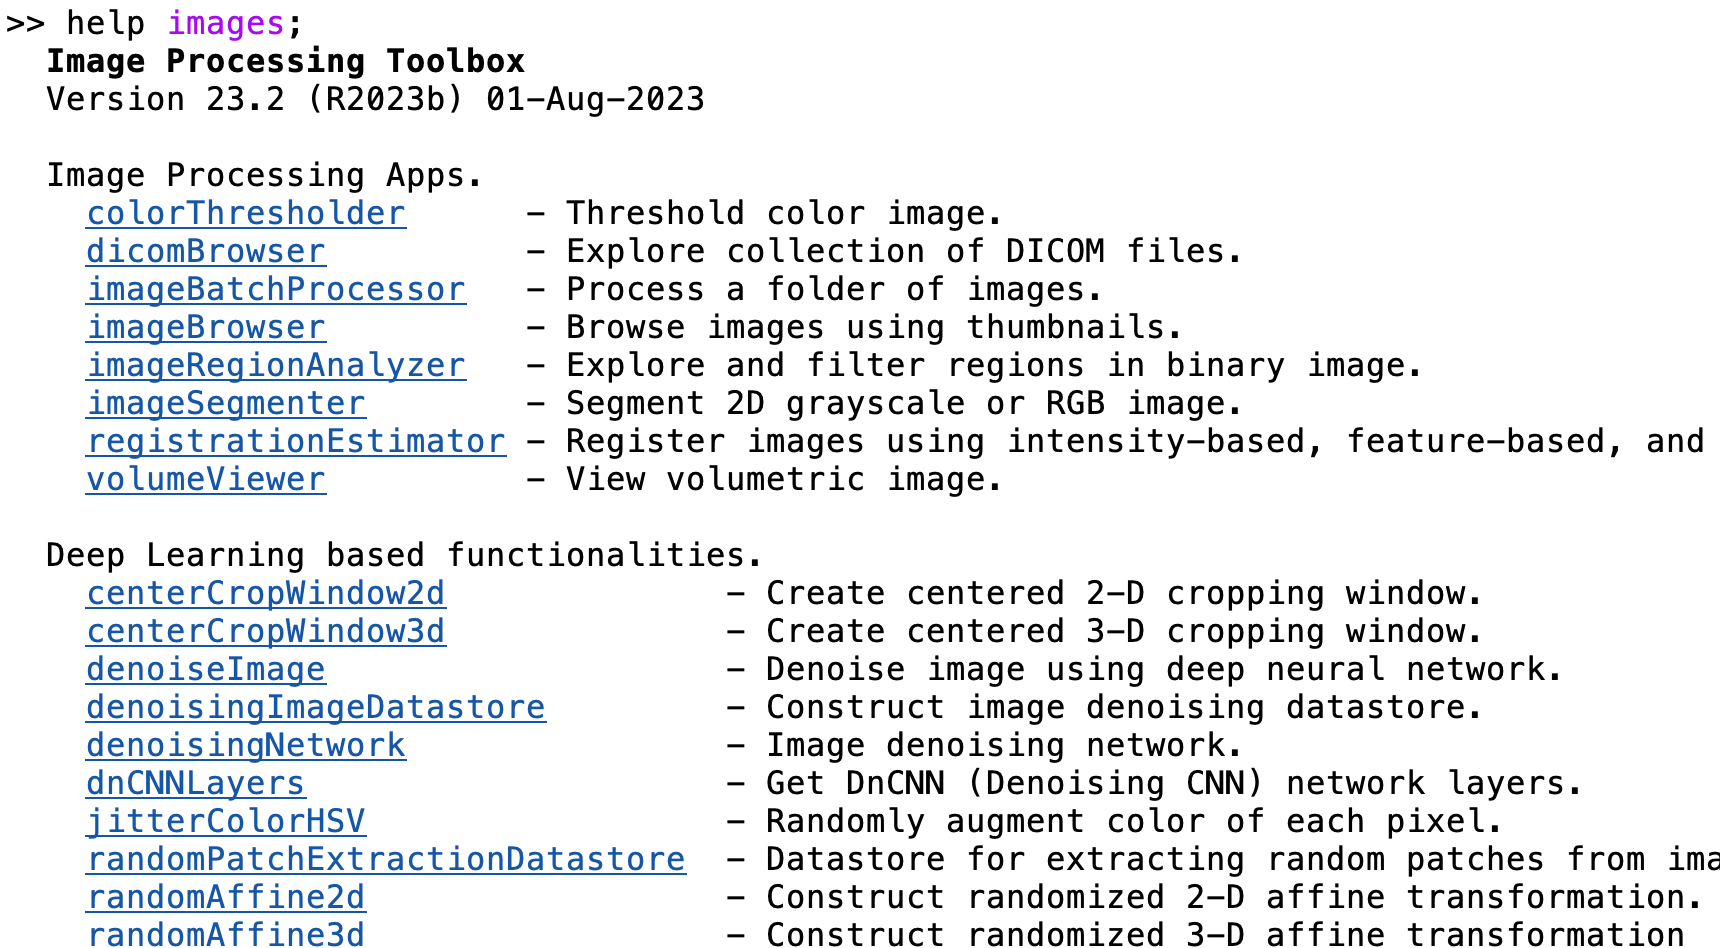
\includegraphics[width=.8\textwidth]{asserts/1_1_help_images.png}
    \caption{
        \texttt{help images} 查看 Image 工具箱内的函数
    }\label{fig:1_1_help_images}
\end{figure}


\subsection{Image file I/O 作图}

首先,通过 \texttt{load('./resource/hall.mat');} 读取图像数据。

值得注意的是,图像的数据类型是 uint8,即无符号 8 位整数,取值范围为 $[0, 255]$。但是在进行数据处理时,通常需要将其转换为 double 类型,即双精度浮点数,否则可能导致不确定的结果;在显示或保存图像时,则需要将其转换为 uint8 类型。这一点在之后的压缩编码等实验中尤为重要。

以图像的中心点为圆心画圆,思路是以图像的中心点为圆心,半径约为图像宽度的一半处画一个圆环。只需要将距中心点距离在外环半径和内环半径之间的像素点的 rgb 值设为 [255, 0, 0] 即可。关键代码如下:

\begin{codeblock}{matlab}
    [rows, cols, ~] = size(img);

    center = [cols / 2, rows / 2];
    radius_outer = min(rows, cols) / 2;  % outer radius
    radius_inner = radius_outer - linewidth;  % inner radius

    [x, y] = meshgrid(1:cols, 1:rows);  % generate meshgrid
    mask = (x - center(1)).^2 + (y - center(2)).^2 <= radius_outer^2 & (x - center(1)).^2 + (y - center(2)).^2 >= radius_inner^2;
    circle = double(img);
    circle(:,:,1) = rgb(1) * mask + circle(:,:,1) .* ~mask;  % set rgb value
    circle(:,:,2) = rgb(2) * mask + circle(:,:,2) .* ~mask;
    circle(:,:,3) = rgb(3) * mask + circle(:,:,3) .* ~mask;

    imshow(uint8(circle));
\end{codeblock}

其中,\texttt{mask} 为一个逻辑矩阵,表示距中心点距离在外环半径和内环半径之间的像素点。\texttt{rgb} 为设定的 rgb 值,\texttt{linewidth} 为环的宽度。该方法封装在 \texttt{plot\_circle} 中。

绘制位图如图 \ref{fig:1_2_circle}。

用类似的方法,可以绘制棋盘。思路是将每个像素的横纵坐标分别整除棋盘格子的边长,相加后对 2 取模,即可得到棋盘格子的颜色。关键代码如下:

\begin{codeblock}{matlab}
    [rows, cols, channels] = size(img);

    [x, y] = meshgrid(1:cols, 1:rows);  % generate meshgrid
    checkerboard = mod(floor((x - 0.5) / length) + floor((y - 0.5) / length), 2);  % 0.5 for better visualization
    mask = repmat(checkerboard, [1, 1, channels]) == 0;  % set rgb to black
    chess = double(img);
    chess(mask) = 0;

    imshow(uint8(chess));
\end{codeblock}

其中,\texttt{checkerboard} 为一个逻辑矩阵,表示棋盘格子的颜色。\texttt{length} 为棋盘格子的边长。该方法封装在 \texttt{plot\_chess} 中。

绘制位图如图 \ref{fig:1_2_chess}。

\begin{figure}[ht]
    \centering
    \begin{subfigure}[b]{0.4\textwidth}
        \centering
        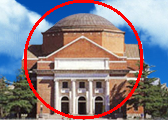
\includegraphics[width=\textwidth]{asserts/1_2_circle.png}
        \caption{
            以图像的中心点为圆心画圆
        }\label{fig:1_2_circle}
    \end{subfigure}
    \hfill
    \begin{subfigure}[b]{0.4\textwidth}
        \centering
        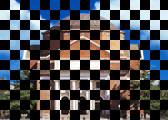
\includegraphics[width=\textwidth]{asserts/1_2_chess.png}
        \caption{
            绘制棋盘
        }\label{fig:1_2_chess}
    \end{subfigure}
    \caption{
        图像作图
    }
\end{figure}

\section{图像压缩编码}

\subsection{DCT 域预处理}

注意到,DCT 同 FFT 类似,满足线性性质,即 $DCT(a \cdot x + b \cdot y) = a \cdot DCT(x) + b \cdot DCT(y)$。
因此,先将图像灰度值减去 128,再进行 DCT 变换,等价于先进行 DCT 变换,再将 DCT 变换后的系数减去全为 128 的矩阵的 DCT 变换。
由于全为 128 的矩阵只包含直流分量,因此其 DCT 变换后只有左上角的系数非零,故只需将左上角的系数减去全为 128 的矩阵的 DCT 变换的直流分量。
同时,在二维 DCT 变换公式中,令 $i=0, j=0$,可得:

\begin{align*}
    F(0, 0) &= \frac{1}{\sqrt{MN}} \sum_{x=0}^{M-1} \sum_{y=0}^{N-1} f(x, y) \cos\left(\frac{(2x+1)0\pi}{2M}\right) \cos\left(\frac{(2y+1)0\pi}{2N}\right) \\
    &= \frac{1}{\sqrt{MN}} \sum_{x=0}^{M-1} \sum_{y=0}^{N-1} f(x, y) \cos(0) \cos(0) \\
    &= \frac{1}{\sqrt{MN}} \sum_{x=0}^{M-1} \sum_{y=0}^{N-1} f(x, y)
\end{align*}

故 DCT 直流分量可以通过计算原图像的均值,并乘以 $\frac{1}{\sqrt{MN}}$ 得到。在本题中,即 $128 * 8 = 1024$。

因此 DCT 在变换域的预处理可以用以下代码实现并验证:

\begin{codeblock}{matlab}
    patch00 = double(hall_gray(1:8, 1:8));
    c_patch00_trans = dct2(patch00);
    c_patch00_trans(1, 1) = c_patch00_trans(1, 1) - 128 * 8;
    c_patch00_ori = dct2(patch00 - 128);
    disp("SSE: " + sum((c_patch00_trans - c_patch00_ori).^2, 'all'));
\end{codeblock}

得到 SSE 为 3.5715e-25,即两种方法得到的 DCT 系数完全一致,验证了此变换域预处理方法的正确性。

\subsection{二维 DCT 实现}

首先计算变换矩阵 D,代码如下:

\begin{codeblock}{matlab}
function D = dct_D(N)
    % Create the 2D DCT matrix
    % N [int]: the size of the matrix
    % return D [2D double]: the DCT matrix
    D = [1 : N - 1]' * [1: 2: 2 * N - 1];
    D = cos(D * pi / (2 * N));
    D = [repmat(sqrt(0.5), [1, N]); D];
    D = D * sqrt(2 / N);
end
\end{codeblock}

通过矩阵运算,避免了显式的循环,提高了运算效率。

接着实现二维 DCT 变换,代码如下:

\begin{codeblock}{matlab}
function C = dct_2(P, s)
    % Perform 2D DCT on the input matrix
    % P [2D double]: the input matrix
    % s [1D int][optional]: the size of the matrix
    % return C [2D double]: the DCT matrix
    [rows, cols] = size(P);
    
    if nargin < 2
        if rows == cols
            D = dct_D(rows);
            C = D * P * D';
        else
            D = dct_D(rows);
            D_T = dct_D(cols)';
            C = D * P * D_T;
        end
    else
        P_padding = zeros(s);
        min_rows = min(rows, s(1));
        min_cols = min(cols, s(2));
        P_padding(1:min_rows, 1:min_cols) = P(1:min_rows, 1:min_cols);
        if s(1) == s(2)
            D = dct_D(s(1));
            C = D * P_padding * D';
        else
            D = dct_D(s(1));
            D_T = dct_D(s(2))';
            C = D * P_padding * D_T;
        end
    end
end
\end{codeblock}

注意到,MATLAB 库提供的 \texttt{dct2} 函数可以处理任意形状的矩阵(并不局限于方阵),并且可以指定变换域的大小,视情况对输入矩阵进行 padding 或 truncation。
因此,我实现的 \texttt{dct\_2} 函数也具有这两个功能,且参数数目可变,输入输出格式与 \texttt{dct2} 完全一致。

特别的,我实现的 \texttt{dct\_2} 函数对方阵进行了优化,避免了两次计算 D 矩阵,提高了运算效率。

下面,我分别对方阵和非方阵的矩阵进行了功能验证,验证代码如下:

\begin{codeblock}{matlab}
patch00 = double(hall_gray(1:8, 1:8));
c_patch00 = dct2(patch00);
c_patch00_ = dct_2(patch00);
disp("SSE: " + sum((c_patch00 - c_patch00_).^2, 'all'));
c_patch00 = dct2(patch00, [6, 10]);
c_patch00_ = dct_2(patch00, [6, 10]);
disp("SSE: " + sum((c_patch00 - c_patch00_).^2, 'all'));
\end{codeblock}

SSE 截图如图 \ref{fig:2_2_sse},验证了 \texttt{dct\_2} 函数的正确性。

\begin{figure}[ht]
    \centering
    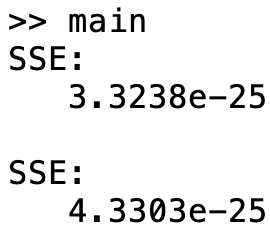
\includegraphics[width=0.25\textwidth]{asserts/2_2_sse.png}
    \caption{
        DCT 正确性验证
    }\label{fig:2_2_sse}
\end{figure}

我还对 \texttt{dct\_2} 函数的运行时间与原 MATLAB 库提供的 \texttt{dct2} 函数进行了比较,两者各运行 100000 次,结果如图 \ref{fig:2_2_time}。

\begin{figure}[ht]
    \centering
    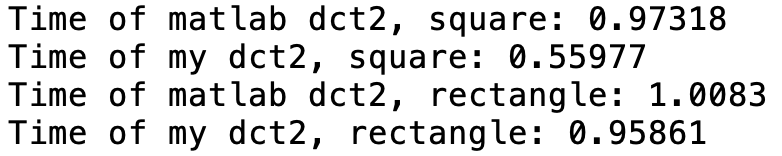
\includegraphics[width=0.6\textwidth]{asserts/2_2_time.png}
    \caption{
        DCT 运行时间比较
    }\label{fig:2_2_time}
\end{figure}

可见,我实现的 \texttt{dct\_2} 函数比 MATLAB 库提供的 \texttt{dct2} 函数更高效,尤其在方阵的情况下,速度提高接近 2 倍。


\subsection{DCT 系数置零}

理论上,DCT 变换得到的系数矩阵左上角代表直流分量,左下代表纵向分量变化的高频分量,右上代表横向变化的高频分量,右下代表横向和纵向变化的高频分量。
因此,若将右侧 4 列置零,主要会损失横向变化的高频分量,横向亮度变化会变模糊。
但由于图像中高频分量的能量较低,因此这种损失对图像的影响较小,视觉效果不会有太大变化。

若将左侧 4 列置零,主要会损失直流分量和纵向分量变化的高频分量。
一方面,纵向亮度变化会变模糊。
另一方面,图像亮度会趋于相同。由于处理前直流分量减去了 128,恢复时要加上 128,故亮度会趋于 128,呈现灰色。
由于人眼对低频分量更敏感,因此这种损失对图像的影响较大,视觉效果上看图像严重受损。

为了验证猜想,我将图片按横纵 8*8 分块,对每个块进行 DCT 变换,并将对应列置零。效果如图 \ref{fig:2_3_image}。

\begin{figure}[ht]
    \centering
    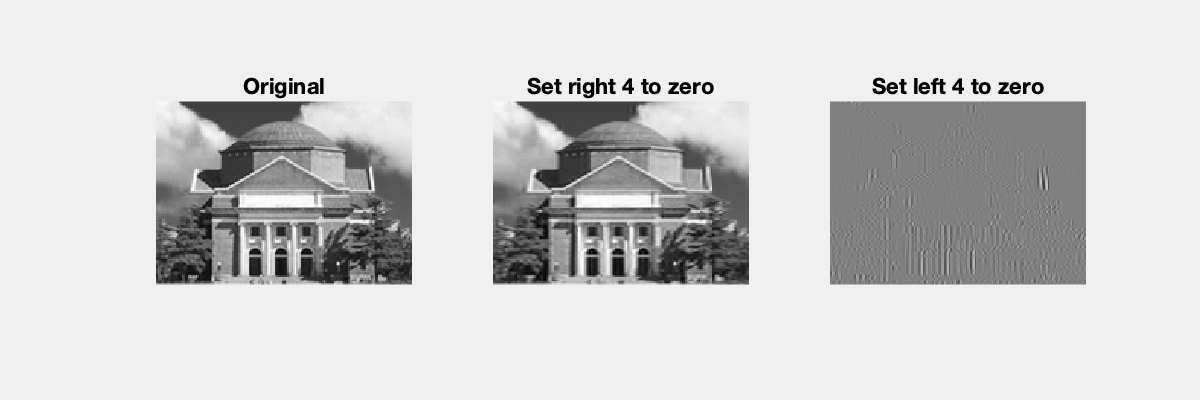
\includegraphics[width=0.8\textwidth]{asserts/2_3_image.png}
    \caption{
        系数置零整体效果
    }\label{fig:2_3_image}
\end{figure}

可见,将左侧 4 列置零后,图像亮度整体受损严重,成为一片灰色。
唯一保留的是横向变化的分量。由于这部分能量较低,呈现零星的纵向纹路。
而将右侧 4 列置零后,图像变化不明显,与理论分析一致。

局部效果如图 \ref{fig:2_3_patch}。
可以看到,将左侧 4 列置零后,直流分量损失严重,局部变成灰色块。
而将右侧 4 列置零后,直接和纵向分量几乎不受影响,但横向变得模糊,呈现条带状。

\begin{figure}[ht]
    \centering
    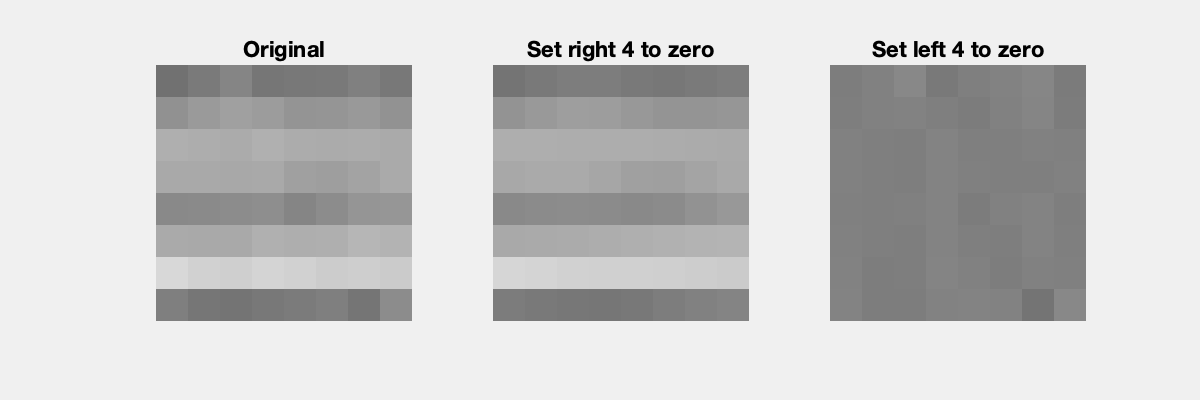
\includegraphics[width=0.8\textwidth]{asserts/2_3_patch.png}
    \caption{
        系数置零局部效果
    }\label{fig:2_3_patch}
\end{figure}

\subsection{DCT 系数矩阵变换}

转置:横向分量与纵向分量交换,直流分量和横纵高频分量不变。注意到:

\begin{align*}
C^T = (DPD^T)^T = DP^TD^T = \text{DCT}(P^T)
\end{align*}

因此,还原出来的图像是原图形的转置,即图像绕左上-右下对角线翻转。

旋转 90 度:左上变左下,低频分量变纵向高频分量;右上变左上,横向高频分量变低频分量。
由于原图像低频能量较高,高频能量较低,因此旋转 90 度后,图像的纵向变化会很剧烈,但整体亮度趋于灰色,严重受损。

旋转 180 度:左上与右下互换,低频分量与横纵高频分量互换,横纵高频分量能量大大增加,直流受损,图像亮度应呈棋盘状剧烈变化。

局部效果如图 \ref{fig:2_4_patch}。

\begin{figure}[ht]
    \centering
    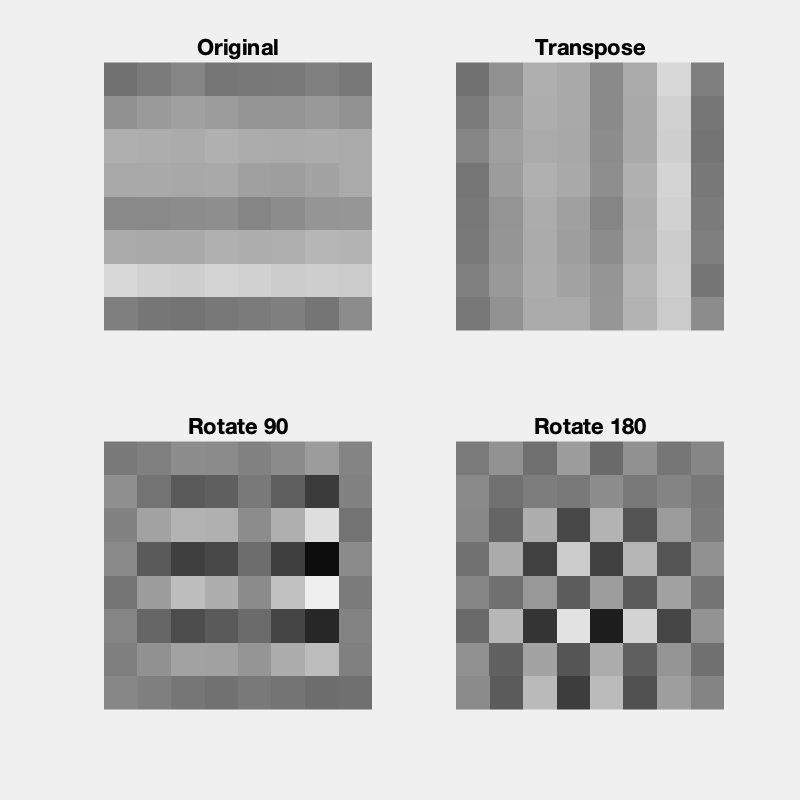
\includegraphics[width=0.6\textwidth]{asserts/2_4_patch.png}
    \caption{
        DCT 系数矩阵变换局部效果
    }\label{fig:2_4_patch}
\end{figure}

可见,转置后恢复的图像确实是原图像的转置,旋转 90 度后图像的纵向变化剧烈,旋转 180 度后图像呈棋盘状,与理论一致。

整体效果如图 \ref{fig:2_4_image}。

\begin{figure}[ht]
    \centering
    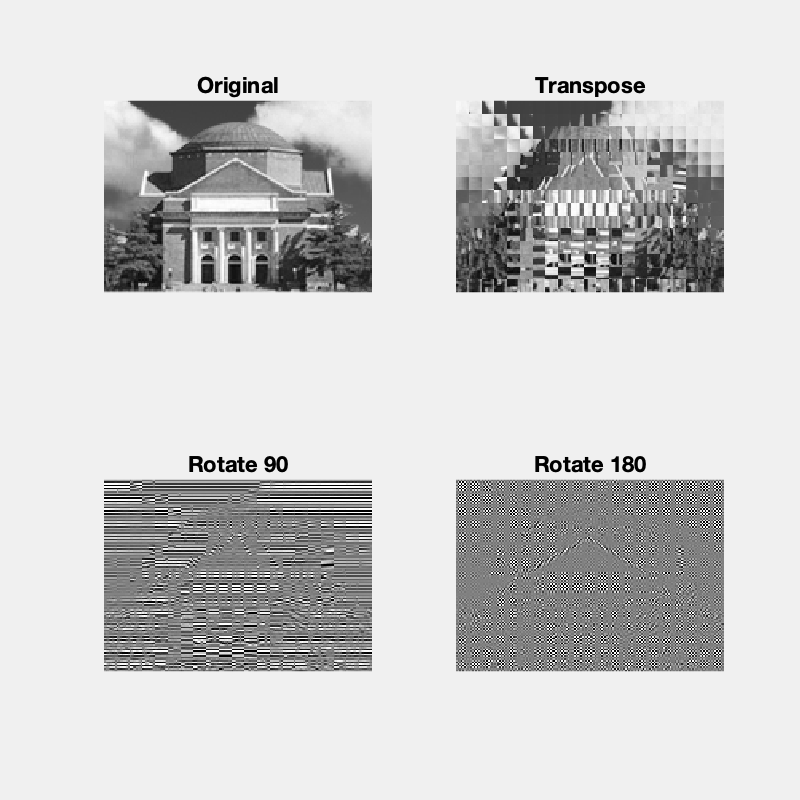
\includegraphics[width=0.75\textwidth]{asserts/2_4_image.png}
    \caption{
        DCT 系数矩阵变换整体效果
    }\label{fig:2_4_image}
\end{figure}

由于图像被分成 8*8 的块,因此转置后图像是大量局部转置按原顺序拼接而成的结果,凌乱中还看得出原图像的大致轮廓,颇有一种抽象油彩画的感觉,也与受损老照片有几份形似。
而旋转 90 度后,则几乎只能看出纵向的剧烈变化,整体严重受损。
旋转 180 度后,图像像多个棋盘拼接而成,形态类似纱布。这些现象均与理论分析一致。

\subsection{差分编码系统}

对于直流分量,通过差分编码后输出为零;对于剧烈变化的高频分量,通过差分编码后能量可能会增加,例如 1, -1, 1, -1, ... 将成为 2, -2, 2, -2, ...。
因此猜想差分编码系统是高通滤波器。

绘制频率响应如图 \ref{fig:2_5_freq}。可见确实是一个高通滤波器。

\begin{figure}[ht]
    \centering
    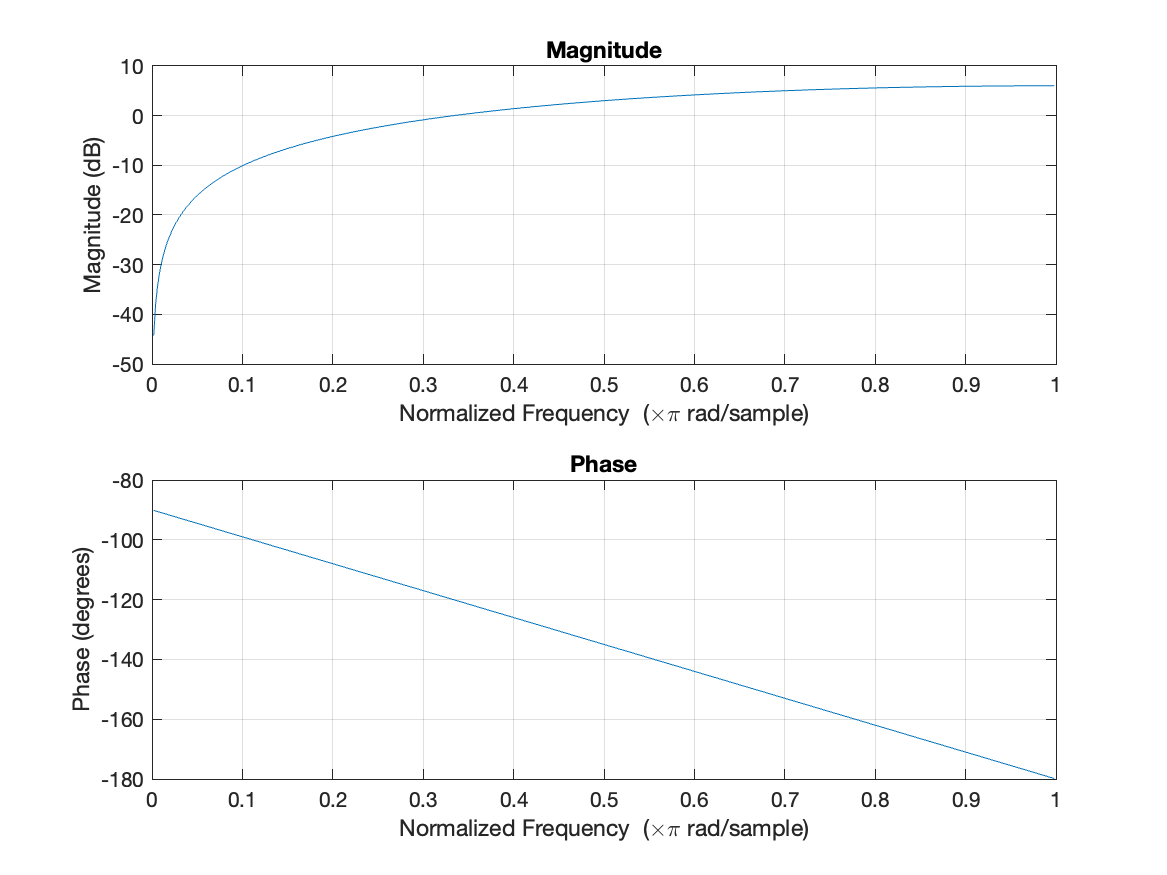
\includegraphics[width=0.6\textwidth]{asserts/2_5_freqz.png}
    \caption{
        差分编码系统频率响应
    }\label{fig:2_5_freq}
\end{figure}

DC 系数先进行差分编码再进行熵编码,说明 DC 系数的低频分量更多。
这样做的好处是,通过差分编码后能有效降低能量,编码时可以节省比特数,在保持信息不丢失的前提下提高压缩率。

\subsection{DC 预测误差与 Category 的关系}

记 DC 预测误差为 $\delta$,类别为 $C$,容易发现,$C = \min(\text{ceil}(\log_2(|\delta| + 1)), 11)$。
这里不用 $\text{floor}$ 是为了避免 $C = 0$ 的情况产生算术溢出,增加 $\min$ 是为了处理预测误差超过预定上下界的情况,提高鲁棒性。

\subsection{Zig-Zag 扫描算法}

一种通用的方法是按 Zig-Zag 扫描顺序将矩阵展开为向量,封装如下:

\begin{codeblock}{matlab}
function o = zig_zag(i)
    [N, M] = size(i);
    o = zeros(1, N * M);
    o(1) = i(1, 1);
    row = 1;
    col = 1;
    flag = 0;  % 1 means row increases and column decreases

    for idx = 2 : N * M
        if col == N && flag == 0
            row = row + 1; flag = 1;
        elseif row == N && flag == 1
            col = col + 1; flag = 0;
        elseif row == 1  && flag == 0
            col = col + 1; flag = 1;
        elseif col == 1  && flag == 1
            row = row + 1; flag = 0;
        elseif flag == 1
            row = row + 1; col = col - 1;
        else
            row = row - 1; col = col + 1;
        end
        o(idx) = i(row, col);
    end
end
\end{codeblock}

上述算法具备很好的通用性,可以处理任意形状的矩阵,但需要二重循环,效率较低。

本题中,由于矩阵是固定的 8*8 的方阵,可以利用查表法,配合矩阵索引,对输入输出索引建立双射关系,提高效率,代码如下:

\begin{codeblock}{matlab}
function o = zig_zag_8_8(i)
    % Perform zig-zag scan on the input matrix, assuming the input is 8x8
    % i [2D double]: the input matrix
    % return o [1D double]: the zig-zag scanned matrix
    idx_matrix = [
        1, 9, 2, 3, 10, 17, 25, 18, ...
        11, 4, 5, 12, 19, 26, 33, 41, ...
        34, 27, 20, 13, 6, 7, 14, 21, ...
        28, 35, 42, 49, 57, 50, 43, 36, ...
        29, 22, 15, 8, 16, 23, 30, 37, ...
        44, 51, 58, 59, 52, 45, 38, 31, ...
        24, 32, 39, 46, 53, 60, 61, 54, ...
        47, 40, 48, 55, 62, 63, 56, 64, ...
    ];
    o = reshape(i, [1, 64]);
    o = o(idx_matrix);
end
\end{codeblock}

下面对 Zig-Zag 扫描算法进行了功能验证,分别选取 8*8 和 9*9 的矩阵对两种算法进行了验证,测试矩阵如下:

\begin{codeblock}{matlab}
input_8_8 = [
    1,  2,  6,  7, 15, 16, 28, 29;
    3,  5,  8, 14, 17, 27, 30, 43;
    4,  9, 13, 18, 26, 31, 42, 44;
    10, 12, 19, 25, 32, 41, 45, 54;
    11, 20, 24, 33, 40, 46, 53, 55;
    21, 23, 34, 39, 47, 52, 56, 61;
    22, 35, 38, 48, 51, 57, 60, 62;
    36, 37, 49, 50, 58, 59, 63, 64;
];
input_9_9 = [
    1,  2,  6,  7, 15, 16, 28, 29, 45;
    3,  5,  8, 14, 17, 27, 30, 44, 46;
    4,  9, 13, 18, 26, 31, 43, 47, 60;
    10, 12, 19, 25, 32, 42, 48, 59, 61;
    11, 20, 24, 33, 41, 49, 58, 62, 71;
    21, 23, 34, 40, 50, 57, 63, 70, 72;
    22, 35, 39, 51, 56, 64, 69, 73, 78;
    36, 38, 52, 55, 65, 68, 74, 77, 79;
    37, 53, 54, 66, 67, 75, 76, 80, 81;
];
\end{codeblock}

预期输出为按 1, 2, 3, ... 的顺序排列的向量。实际输出符合预期(8*8 的如图 \ref{fig:2_7_zigzag88},受限于篇幅,9*9 的不再展示,感兴趣的可以自行验证)。

\begin{figure}[ht]
    \centering
    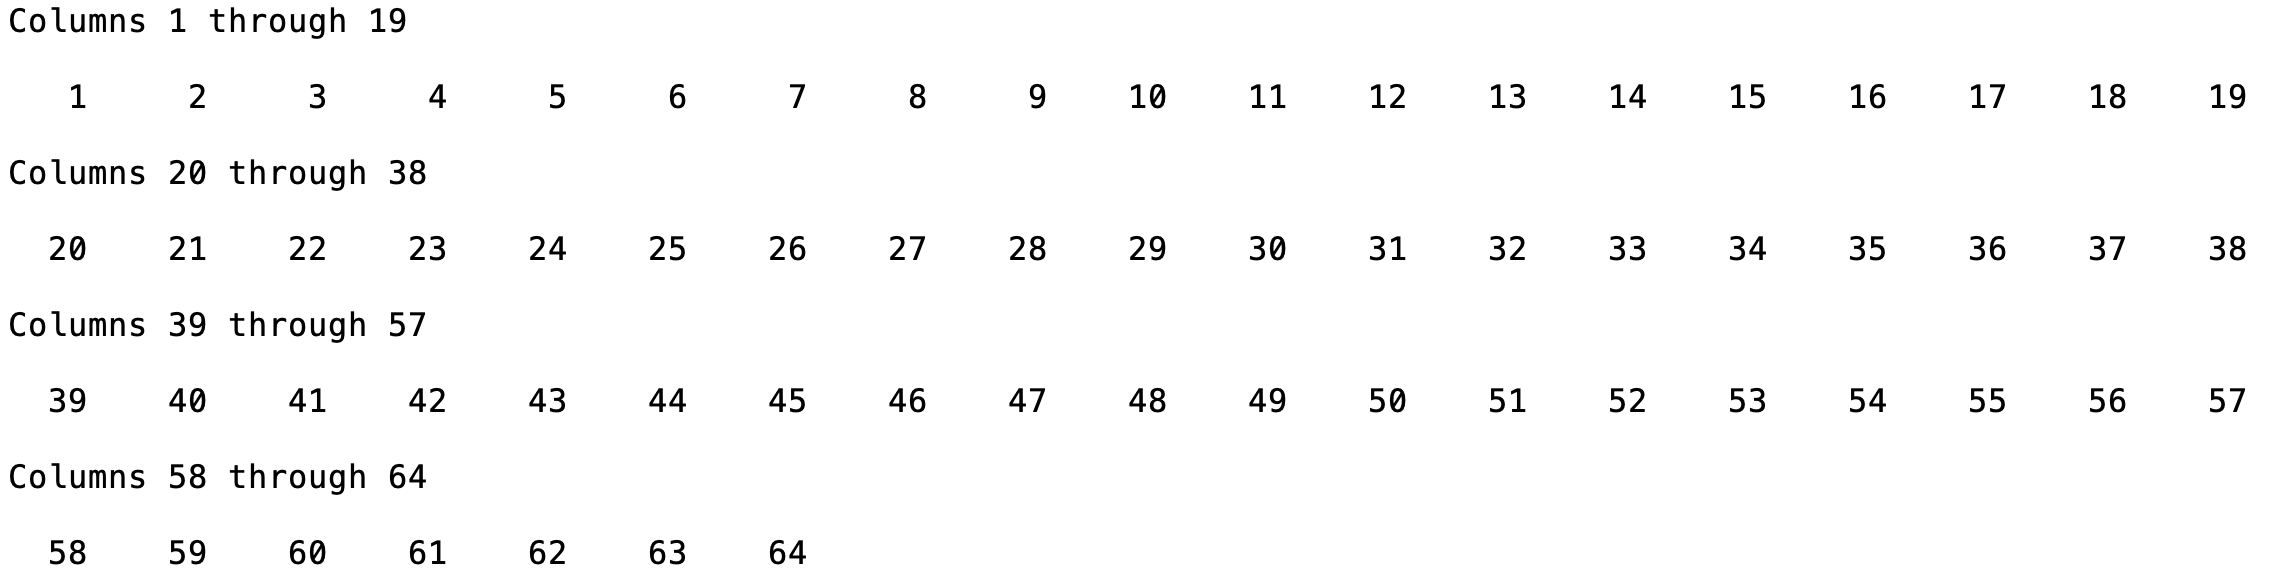
\includegraphics[width=0.75\textwidth]{asserts/2_7_zigzag88.png}
    \caption{
        Zig-Zag 扫描算法功能验证
    }\label{fig:2_7_zigzag88}
\end{figure}

\subsection{分块、DCT 与量化}\label{sec:2_8}

可以利用 MATLAB 的矩阵运算功能和 \texttt{blockproc} 方法高效实现,关键代码如下:

\begin{codeblock}{matlab}
function o = blockproc_8_8(i, func, varargin)
    o = blockproc(i, [8, 8], @(block) func(block.data, varargin{:}), 'PadPartialBlocks', true);
end

[rows, cols] = size(i);
C = blockproc_8_8(double(i) - 128, @dct2);  % DCT
Q = blockproc_8_8(C, @(x) round(x ./ QTAB));  % Quantization
Z = blockproc_8_8(Q, @(x) zig_zag_8_8(x));  % Zig-zag scan
Z = reshape(Z.', [64, ceil(rows / 8) * ceil(cols / 8)]);  % Reshape
\end{codeblock}

其中,\texttt{blockproc\_8\_8} 函数是对 \texttt{blockproc} 针对 8*8 分块的进一步封装,将在之后被多次调用,提高了代码的简洁性。

\subsection{JPEG 编码}

首先,定义十进制数转二进制数的函数,其中负数用 1 补码表示:

\begin{codeblock}{matlab}
function o = dec2bin_arr(i)
    if i ~= 0
        o = dec2bin(abs(i)) - '0';
        if i < 0
            o = ~o;
        end
    else
        o = [];
    end
end
\end{codeblock}

量化后的系数矩阵 Z 已由 \ref{sec:2_8} 中的代码得到,接下来对其直流分量进行差分编码和霍夫曼编码并转化为二进制码流,关键代码如下:

\begin{codeblock}{matlab}
DC = Z(1, :);
DC_diff = [DC(1), DC(1 : end - 1) - DC(2 : end)];
DC_cata = min(ceil(log2(abs(DC_diff) + 1)), 11);
get_code_and_mag_dc = @(cata, diff) [DCTAB(cata + 1, 2 : DCTAB(cata + 1, 1) + 1), dec2bin_arr(diff)];
DC_stream = cell2mat(arrayfun(@(cata, diff) get_code_and_mag_dc(cata, diff), DC_cata, DC_diff, 'UniformOutput', false));
\end{codeblock}

接着对交流分量进行游程编码和霍夫曼编码,关键代码如下:

\begin{codeblock}{matlab}
AC = Z(2 : end, :);
AC_size = min(ceil(log2(abs(AC) + 1)), 10);
AC_stream = [];
EOB = [1 0 1 0];  % End of block
ZRL = [1 1 1 1 1 1 1 1 0 0 1];  % Zero run length
get_code_and_mag_ac = @(run, size, amp) [ACTAB(run * 10 + size, 4 : ACTAB(run * 10 + size, 3) + 3), dec2bin_arr(amp)];
for idx = 1 : size(AC, 2)
    num_zero = 0;
    for jdx = 1 : size(AC, 1)
        if AC(jdx, idx) == 0
            num_zero = num_zero + 1;
        else
            if num_zero > 15
                AC_stream = [AC_stream, repmat(ZRL, 1, floor(num_zero / 16))];
                num_zero = mod(num_zero, 16);
            end
            AC_stream = [AC_stream, get_code_and_mag_ac(num_zero, AC_size(jdx, idx), AC(jdx, idx))];
            num_zero = 0;
        end
    end
    AC_stream = [AC_stream, EOB];
end
\end{codeblock}

最后保存 DC 码流、AC 码流、图像大小。完整代码位于 \texttt{src/jpeg\_encode.m}。

\subsection{计算压缩比}

将原图像与码流长度单位统一为 bit。由于原图像数据类型为 uint8,故需将面积乘以 8。代码如下:

\begin{codeblock}{matlab}
disp("Compression ratio: " + (8 * rows * cols) / (length(DC_stream) + length(AC_stream)));
\end{codeblock}

得到压缩比为 6.4247

\subsection{JPEG 解码}

同样定义二进制数转十进制数的函数,其中负数用 1 补码表示:

\begin{codeblock}{matlab}
function o = bin_arr2dec(i)
    if isempty(i)
        o = 0;
    else
        if i(1) == 0
            i = ~i;
            o = -bin2dec(num2str(i));
        else
            o = bin2dec(num2str(i));
        end
    end
end
\end{codeblock}

为对霍夫曼编码进行解码,构建霍夫曼树。霍夫曼树为一结构体,包含左右子树及对应 symbol。构造过程如下:

\begin{codeblock}{matlab}
function tree = addSymbolToTree(tree, code, symbol)
    if isempty(code)
        tree.symbol = symbol;
        return;
    end
    if code(1) == 0
        if isempty(fieldnames(tree.left))
            tree.left = struct('symbol', NaN, 'left', struct(), 'right', struct());
        end
        tree.left = addSymbolToTree(tree.left, code(2 : end), symbol);
    else
        if isempty(fieldnames(tree.right))
            tree.right = struct('symbol', NaN, 'left', struct(), 'right', struct());
        end
        tree.right = addSymbolToTree(tree.right, code(2 : end), symbol);
    end
end
\end{codeblock}

对 DC 霍夫曼编码构造霍夫曼树:

\begin{codeblock}{matlab}
DC_huffmanTree = struct('symbol', NaN, 'left', struct(), 'right', struct());
for idx = 1:size(DCTAB, 1)
    DC_huffmanTree = addSymbolToTree(DC_huffmanTree, DCTAB(idx, 2 : DCTAB(idx, 1) + 1), idx - 1);
end
\end{codeblock}

对 DC 码流进行解码并反差分,结果保存在矩阵 Z 的第一行。关键代码如下:

\begin{codeblock}{matlab}
    Z = zeros(64, ceil(rows / 8) * ceil(cols / 8));

    DC = [];
    DC_huffman_pointer = DC_huffmanTree;
    idx = 1;
    while idx <= size(DC_stream, 2)
        DC_code = DC_stream(idx);
        if DC_code == 0
            DC_huffman_pointer = DC_huffman_pointer.left;
        else
            DC_huffman_pointer = DC_huffman_pointer.right;
        end
        idx = idx + 1;
        if ~isnan(DC_huffman_pointer.symbol)
            DC_cata = DC_huffman_pointer.symbol;
            DC = [DC, bin_arr2dec(DC_stream(idx : idx + DC_cata - 1))];
            DC_huffman_pointer = DC_huffmanTree;
            idx = idx + DC_cata;
        end
    end

    for idx = 2 : size(DC, 2)
        DC(idx) = DC(idx - 1) - DC(idx);
    end
    Z(1, :) = DC;
\end{codeblock}

对 AC 霍夫曼编码构造霍夫曼树,与 DC 类似,不再赘述。

对 AC 码流进行解码,结果保存在矩阵 Z 的第二行至最后,格式与编码前一致。关键代码如下:

\begin{codeblock}{matlab}
AC = [];
AC_huffman_pointer = AC_huffmanTree;
idx = 1;
patch_idx = 1;
while idx <= size(AC_stream, 2)
    AC_code = AC_stream(idx);
    if AC_code == 0
        AC_huffman_pointer = AC_huffman_pointer.left;
    else
        AC_huffman_pointer = AC_huffman_pointer.right;
    end
    idx = idx + 1;
    if ~isnan(AC_huffman_pointer.symbol)
        AC_run = AC_huffman_pointer.symbol(1);
        AC_size = AC_huffman_pointer.symbol(2);
        if AC_run == 0 && AC_size == 0
            Z(2 : size(AC, 1) + 1, patch_idx) = AC;
            AC = [];
            patch_idx = patch_idx + 1;
        else
            AC = [AC; zeros(AC_run, 1); bin_arr2dec(AC_stream(idx : idx + AC_size - 1))];
            idx = idx + AC_size;
        end
        AC_huffman_pointer = AC_huffmanTree;
    end
end
\end{codeblock}

最后,对 DCT 系数矩阵进行逆量化和逆 DCT 变换,得到原图像:

\begin{codeblock}{matlab}
Z = reshape(Z, [64 * ceil(cols / 8), ceil(rows / 8)]).';
Q = blockproc(Z, [1, 64], @(block) zag_zig_8_8(block.data));
C = blockproc_8_8(Q, @(x) x .* QTAB);
o = blockproc_8_8(C, @idct2) + 128;
o = uint8(o(1:rows, 1:cols));
\end{codeblock}

其中,\texttt{zag\_zig\_8\_8} 函数是 \texttt{zig\_zag\_8\_8} 函数的逆操作,将 Zig-Zag 扫描的结果还原为 8*8 的矩阵,同样采用查表法,不再赘述。
完整代码位于 \texttt{src/jpeg\_decode.m}。

对编码、解码进行测试,结果如图 \ref{fig:2_11_decode}。可以看到,解码后的图像与原图像视觉效果几乎完全一致,说明 JPEG 编码解码过程正确。

\begin{figure}[ht]
    \centering
    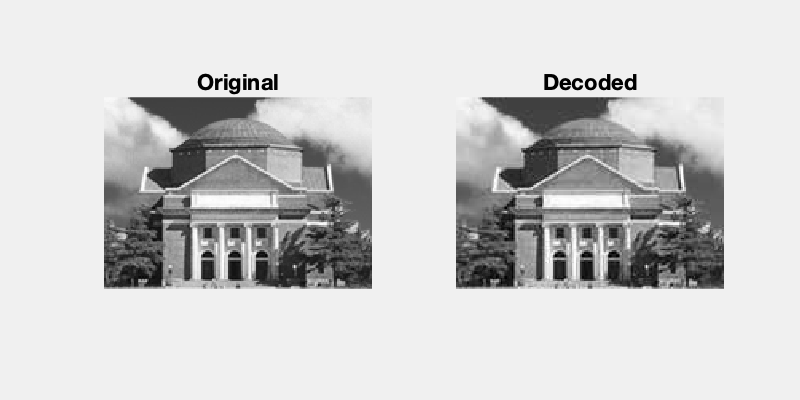
\includegraphics[width=0.8\textwidth]{asserts/2_11_decode.png}
    \caption{
        JPEG 编码解码测试
    }\label{fig:2_11_decode}
\end{figure}

仔细观察图 \ref{fig:2_11_decode},可以发现,解码后的图像存在较明显的块状效应(特别是在白云附近),这是因为 JPEG 编码过程中对图像进行了分块处理,导致边界处的块与块之间存在不连续性。
同时,图像的细节部分也受到了一定程度的模糊,例如亮度变化剧烈的地方,这是量化的结果。

下面用 PSNR 评价解码后的图像与原图像的相似度:

\begin{codeblock}{matlab}
function PSNR = cal_PSNR(ori, img)
    MSE = sum((double(ori) - double(img)).^2, 'all') / numel(ori);
    PSNR = 10 * log10(255^2 / MSE);
end
\end{codeblock}

得到 PSNR 为 31.1874 dB,说明解码后的图像与原图像的相似度较高。

\subsection{量化步长减小一半}

将量化步长减小一半,即 QTAB 中的每个元素除以 2,重新进行 JPEG 编码解码,重新计算压缩比与 PSNR,结果如图 \ref{fig:2_12_res}。

\begin{figure}[ht]
    \centering
    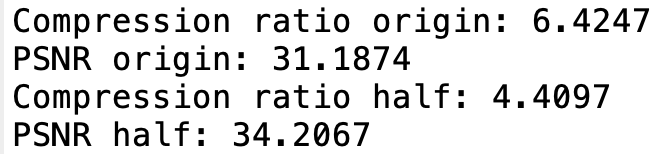
\includegraphics[width=0.5\textwidth]{asserts/2_12_res.png}
    \caption{
        量化步长减小一半与原结果的比较
    }\label{fig:2_12_res}
\end{figure}

可见,压缩比由 6.4247 降低到了 4.4097,PSNR 由 31.1874 dB 提高到了 34.2067 dB。
原因可能在于,量化步长减小后,量化精度提高,高频分量的细节更多地保留了下来,因此 PSNR 提高。
但由于量化步长减小,量化后的系数更大,导致码流长度增加,压缩比降低。

视觉效果如图 \ref{fig:2_12_decode},与原量化步长相比,变化不明显。

\begin{figure}[ht]
    \centering
    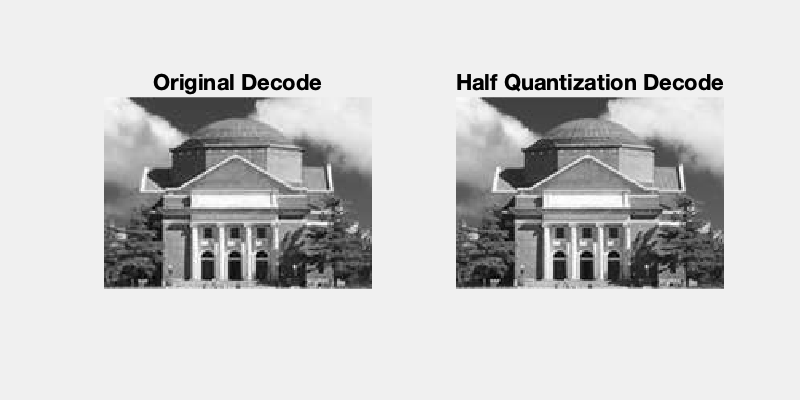
\includegraphics[width=0.8\textwidth]{asserts/2_12_decode.png}
    \caption{
        量化步长减小一半与原结果解码图像比较
    }\label{fig:2_12_decode}
\end{figure}

\subsection{雪花图像 JPEG 编解码}

解码图像与指标如图 \ref{fig:2_13_decode} 与 \ref{fig:2_13_res}。相比大礼堂图像,雪花图像的压缩比较低、PSNR 较低,视觉效果细节上失真较多。
这可能是因为雪花图像的细节更多,高频分量更多,量化后数值较大,压缩比较低;同时,高频分量量化系数较大,细节丢失较多,PSNR 较低。

\begin{figure}[ht]
    \centering
    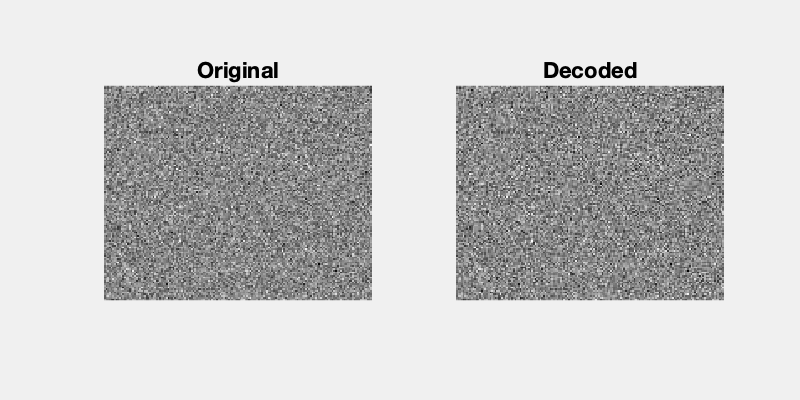
\includegraphics[width=0.8\textwidth]{asserts/2_13_decode.png}
    \caption{
        雪花图像 JPEG 解码图像
    }\label{fig:2_13_decode}
\end{figure}

\begin{figure}[ht]
    \centering
    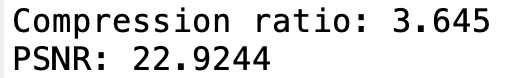
\includegraphics[width=0.4\textwidth]{asserts/2_13_res.png}
    \caption{
        雪花图像 JPEG 编解码结果
    }\label{fig:2_13_res}
\end{figure}

\section{信息隐藏}

\subsection{空域隐藏}

将信息隐藏在图像的最低有效位,关键代码如下:

\begin{codeblock}{matlab}
% encode
i = bitset(i, 1, hidden_info);
% decode
hidden_info = logical(bitget(o, 1));
\end{codeblock}

对大礼堂图像进行信息隐藏,隐藏信息分别取 01 随机序列、全 1 序列、全 0 序列。
隐藏信息后的图像如图 \ref{fig:3_1_decode},解码准确率如图 \ref{fig:3_1_res}。

\begin{figure}[ht]
    \centering
    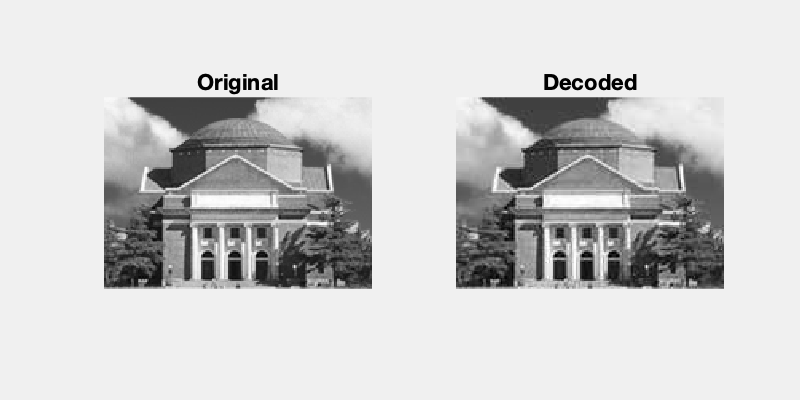
\includegraphics[width=0.8\textwidth]{asserts/3_1_decode.png}
    \caption{
        空域隐藏信息后的图像
    }\label{fig:3_1_decode}
\end{figure}

\begin{figure}[ht]
    \centering
    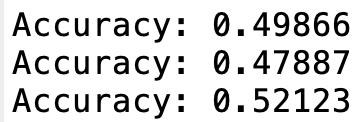
\includegraphics[width=0.4\textwidth]{asserts/3_1_res.png}
    \caption{
        空域隐藏信息解码准确率
    }\label{fig:3_1_res}
\end{figure}

结果表明,图像观感上几乎无失真。但无论隐藏信息是 01 随机序列(高频分量较多)、全 1 序列(直流)还是全 0 序列,解码准确率均在 50\%,附近。
这说明空域隐藏信息的方法在 JPEG 编码下几乎无法保留任何信息,不适合信息隐藏。原因在于,JPEG 编码过程中,对图像进行了量化,导致隐藏信息的最低有效位被破坏,无法准确提取。

为了方便代码复用,空域隐藏的代码写进了 JPEG 编解码方法中(\texttt{src/jpeg\_encode.m} 与 \texttt{src/jpeg\_decode.m}),调用时传入额外的参数 \texttt{enc\_method}、\texttt{dec\_method} 与 \texttt{hidden\_info} 即可,具体实现及用法见代码。
之后的其它信息隐藏方法同样写进了 JPEG 编解码方法中,不再赘述。

\subsection{DCT 域隐藏}

信息隐藏在每个 DCT 系数的最低有效位,关键代码如下:

\begin{codeblock}{matlab}
% encode
Q = double(bitset(int64(Q), 1, hidden_info));
% decode
hidden_info = logical(bitget(int64(Q), 1));
\end{codeblock}

信息隐藏在部分系数的最低位。与隐藏在所有系数的最低位相比,隐藏在部分系数的最低位,可以减小隐藏信息对图像的影响,提高隐藏信息的隐蔽性。
为了最小化隐藏信息对图像的影响,我选取量化矩阵 QTAB 中系数最小的位置用来隐藏信息。
这是因为,量化系数越小,最低位等量的变化(加减 1)所对原 DCT 系数的影响越小,失真也越小。
关键代码如下。其中量化矩阵系数最小的位置由计算得到,具备很好的通用性。同时,由于各列中系数最小的位置是固定的,可以用矩阵运算处理。

\begin{codeblock}{matlab}
% encode
[~, min_QTAB_idx] = min(QTAB(:));
idx_matrix = zeros(8, 8);
idx_matrix(mod(min_QTAB_idx - 1, 8) + 1, floor((min_QTAB_idx - 1) / 8) + 1) = 1;
[~, min_QTAB_idx] = max(zig_zag_8_8(idx_matrix));
Z(min_QTAB_idx, :) = double(bitset(int64(Z(min_QTAB_idx, :)), 1, hidden_info));
% decode
[~, min_QTAB_idx] = min(QTAB(:));
idx_matrix = zeros(8, 8);
idx_matrix(mod(min_QTAB_idx - 1, 8) + 1, floor((min_QTAB_idx - 1) / 8) + 1) = 1;
[~, min_QTAB_idx] = max(zig_zag_8_8(idx_matrix));
hidden_info = logical(bitget(int64(Z(min_QTAB_idx, :)), 1));
\end{codeblock}

信息隐藏在最后一个非零系数之后,用 1 表示 1,-1 表示 0。由于各列非零系数并不固定,因此需要逐列处理,关键代码如下:

\begin{codeblock}{matlab}
% encode
hidden_info = double(hidden_info);
hidden_info(hidden_info == 0) = -1;
for idx = 1 : min(size(Z, 2), length(hidden_info))
    non_zero_indices = find(Z(:, idx));
    if ~isempty(non_zero_indices)
        last_non_zero_idx = non_zero_indices(end);
        if last_non_zero_idx == size(Z, 1)
            Z(last_non_zero_idx, idx) = hidden_info(idx);
        else
            Z(last_non_zero_idx + 1, idx) = hidden_info(idx);
        end
    else
        Z(1, idx) = hidden_info(idx);
    end
end
% decode
hidden_info = logical(zeros(1, size(Z, 2)));
for idx = 1 : size(Z, 2)
    non_zero_indices = find(Z(:, idx));
    if ~isempty(non_zero_indices)
        last_non_zero_idx = non_zero_indices(end);
        hidden_info(idx) = Z(last_non_zero_idx, idx) == 1;
    end
end
\end{codeblock}

对大礼堂图像进行信息隐藏,隐藏信息取 01 随机序列。隐藏信息后的图像如图 \ref{fig:3_2_decode},解码准确率与 PSNR 如图 \ref{fig:3_2_res}。

\begin{figure}[ht]
    \centering
    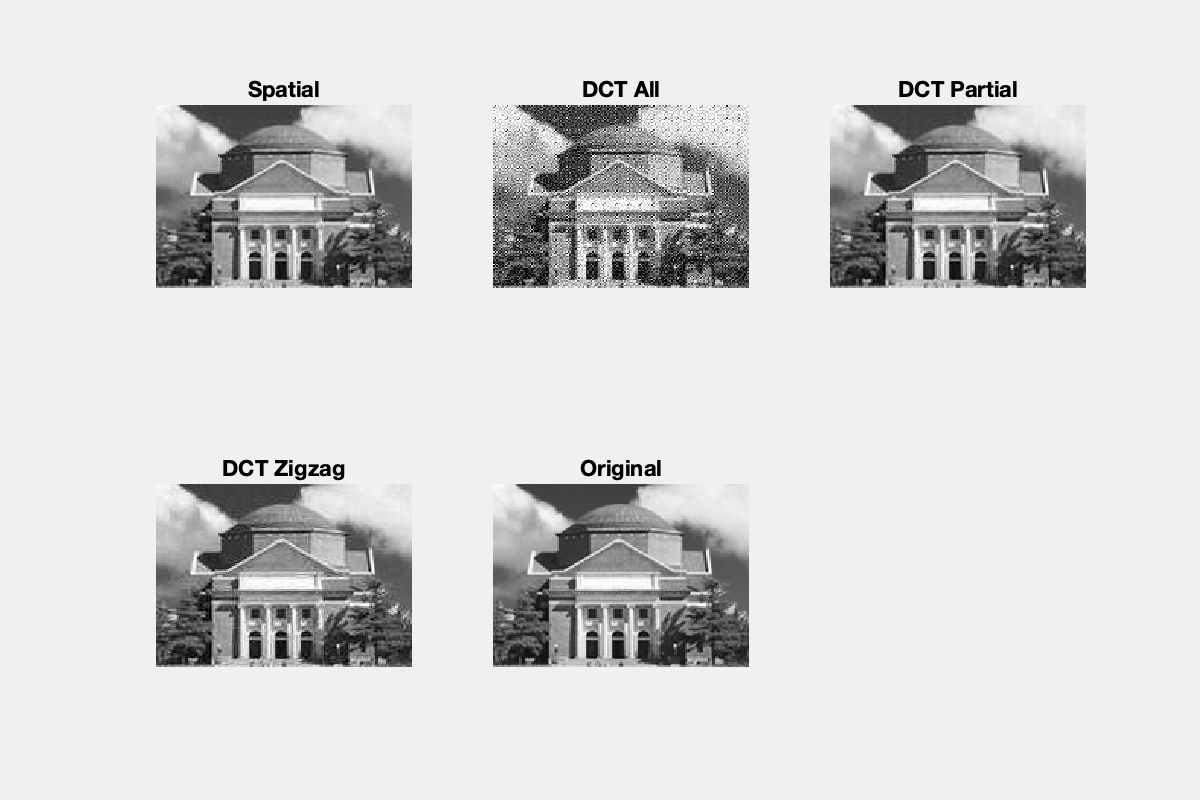
\includegraphics[width=0.8\textwidth]{asserts/3_2_decode.png}
    \caption{
        DCT 域隐藏信息后的图像
    }\label{fig:3_2_decode}
\end{figure}

\begin{figure}[ht]
    \centering
    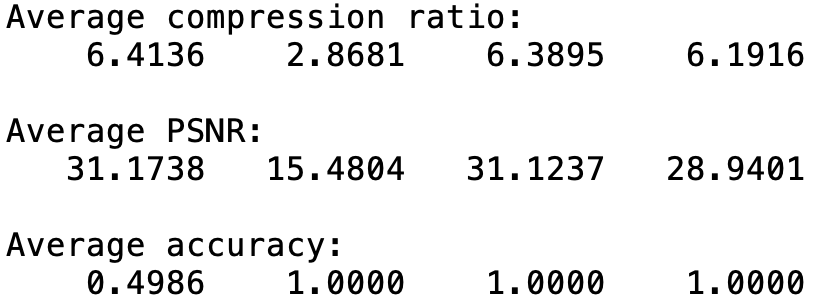
\includegraphics[width=0.7\textwidth]{asserts/3_2_res.png}
    \caption{
        DCT 域隐藏信息解码准确率 \& PSNR \\
        从左到右分别为空域隐藏、DCT 域全部最低位隐藏、DCT 域部分最低位隐藏、DCT 域最后非零系数后隐藏\\
    }\label{fig:3_2_res}
\end{figure}

可见,DCT 域三种信息隐藏的方法均能完整地保留信息,解码准确率均为 100\%。

从观感上,DCT 域全部最低位隐藏失真较明显,高频分量变得很多。
原因在于此方法对每个系数的最低位进行了修改,而高频分量量化系数较大,最低位的变化对原系数的影响较大。
同时,原始图像的高频分量较少,量化后多为 0,此时由 0 变 1 导致图像高频分量显著增加,失真明显。

其它几种量化方法对图像的影响较小。
其中,压缩率与 PSNR 最高的是第二种 DCT 域部分最低位隐藏。
这可能是因为隐藏信息的位置被选取得当(即量化系数最小),对图像的影响最小。

值得注意的是,最后一种(DCT 域最后非零系数后)隐藏的方法是可以几乎完美地恢复出原始图像的(将最低非零系数置零即可),前提是知道图像采用的是这种隐藏信息的技术。
但这种恢复方法不应出现在解码器中。毕竟用于隐藏信息的图像本质上是用来给别人看的,别人大概率不知道隐藏信息的方法。因此没有太多实际意义。

\subsection{新的信息隐藏方法}

由之前的分析可知,选取量化系数最小的位置隐藏信息,可以很好地减小隐藏信息对图像的影响,提高隐藏信息的隐蔽性。
但缺点在于,这种方法每 64 个系数只能隐藏 1 位信息,隐藏效率较低。同时,上述隐藏信息的方法形式过于简单,容易被攻击者破解。

因此一种折中的思路是,根据隐藏信息的长度,动态选取若干个量化系数最小的位置隐藏信息。每个分块的隐藏信息的长度由前一个分块的隐藏信息决定(例如隐藏信息的长度为前一个分块的最后两个隐藏信息所表示的数 + 3)。
这种方法可以在保证隐藏信息对图像影响较小的前提下,提高隐藏效率。同时,由于后一个分块的隐藏信息选取位置依赖于前一个分块的隐藏信息,排除了攻击者对单个分块隐藏格式暴力破解的可能性,大大提高了破解的复杂度。


\section{人脸检测}

\subsection{训练人脸标准}

由于我们采用的标准是各种色彩占图片的比例,即对图片大小进行了归一化,因此无需将图片调整为相同大小。

L 越大,对颜色的区分度可能更精细。下面对 L = 3, 4, 5 进行训练。
首先定义将 RGB 值转化为对应标量的函数:

\begin{codeblock}{matlab}
function num = rgb2scalar(rgb, L)
    num = bitshift(rgb(1), L - 8) * (2 ^ (2 * L)) + bitshift(rgb(2), L - 8) * (2 ^ L) + bitshift(rgb(3), L - 8);
end
\end{codeblock}

接着定义训练函数,返回特征向量,关键代码如下:

\begin{codeblock}{matlab}
function v = train(imgs, L)
    vals = zeros(1, 2 ^ (3 * L));
    edge = -0.5 : 1 : 2 ^ (3 * L) - 0.5;
    for idx = 1:length(imgs)
        img = imgs{idx};
        [h, w, ~] = size(img);
        img = reshape(img, [h * w, 3]);
        val = zeros(1, h * w);
        for i = 1 : h * w
            val(i) = rgb2scalar(int64(img(i, :)), L);
        end
        vals = vals + histcounts(val, edge) / (h * w);
    end
    v = vals / length(imgs);
end
\end{codeblock}

注意这里预定义了 \texttt{val = zeros(1, h * w);} 而不是采用 \texttt{val = []; val = [val, ...]} 的方法,这是因为 \texttt{val = [val, ...]} 这种写法会导致每次迭代都会重新分配内存,效率较低。
这种速度的差异在之后的人脸识别程序中会较明显。

特征向量如图 \ref{fig:4_1_bar}。
可以看到,L 越大,特征向量的维度越高,对颜色的区分度越精细;L 较小时,更多相似的颜色被合并到了一起。
可以认为,较小的 L 得到的特征向量是较大的 L 的特征向量对应周围密度值的求和。

\begin{figure}[ht]
    \centering
    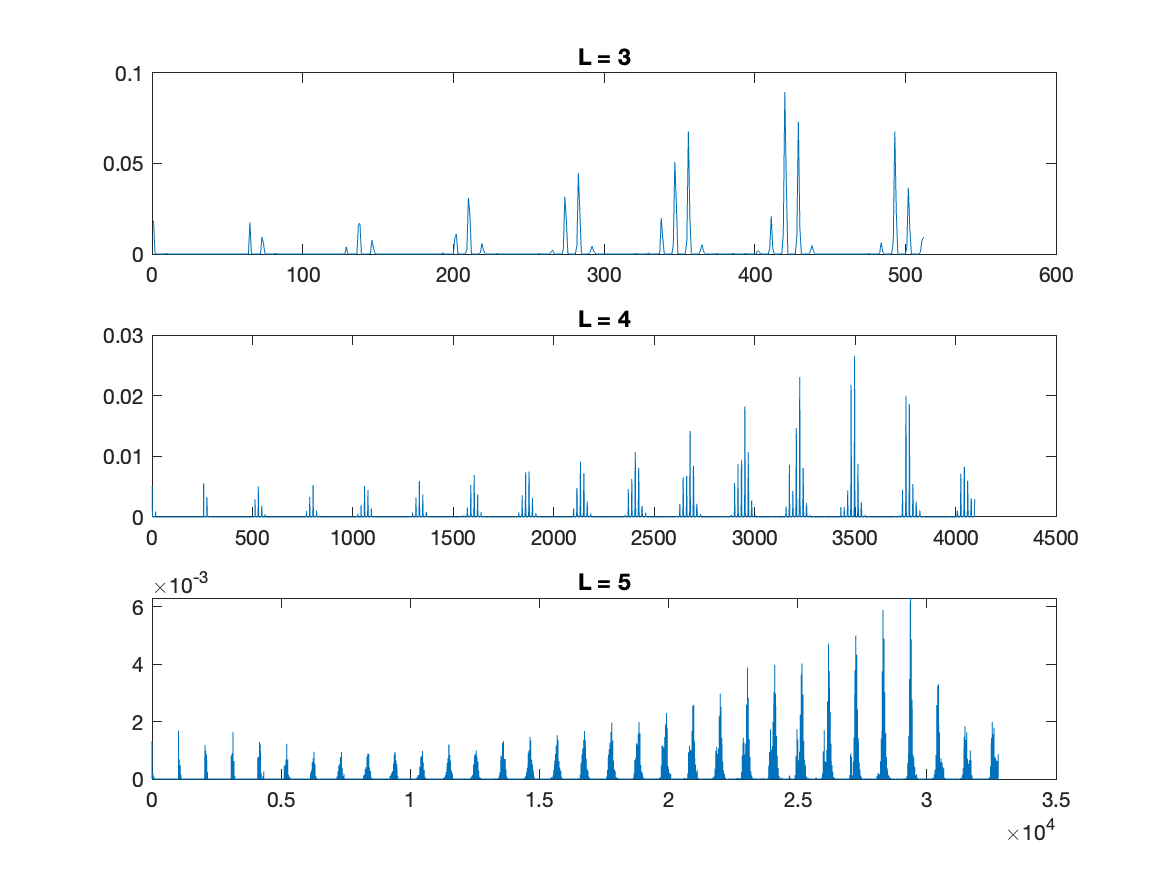
\includegraphics[width=0.8\textwidth]{asserts/4_1_bar.png}
    \caption{
        L = 3, 4, 5 的特征向量
    }\label{fig:4_1_bar}
\end{figure}

\subsection{人脸检测}

算法如下,基本思路是:

\begin{enumerate}
    \item 首先选取大小合适的窗口及步长,对每个窗口进行特征提取,然后与训练得到的特征向量进行比较,若相似度超过阈值,则认为检测到人脸。
    \item 接着对小窗口进行合并。合并的准则是,若任意两个窗口的重叠面积占较小窗口的比例超过阈值,则认为两个窗口重叠,将其合并。
    \item 然后,将面积较小窗口视为噪声,并剔除。
    \item 重复上述步骤,直到不再有窗口合并。
    \item 在第一轮循环中,由于存在大量可能是噪声的小窗口,因此重叠判定的阈值较高,为 0.5,剔除阈值较高,为窗口面积平均值的 1 倍;在之后的循环中,降低重叠判定的阈值为 0.25,降低剔除判定的阈值为窗口面积平均值的 0.5 倍,以更好地保留并合并人脸处的窗口。
\end{enumerate}

关键代码如下:

\begin{codeblock}{matlab}
function face_recognition(img, height, width, step_h, step_w, L, v, threshold)
    [h, w, ~] = size(img);
    edge = -0.5 : 1 : 2 ^ (3 * L) - 0.5;
    position = [];
    % find small windows
    for i = 1 : step_h : h - height + 1
        for j = 1 : step_w : w - width + 1
            window = img(i : i + height - 1, j : j + width - 1, :);
            [h_, w_, ~] = size(window);
            window = reshape(window, [h_ * w_, 3]);
            val = zeros(1, h_ * w_);
            for k = 1 : h_ * w_
                val(k) = rgb2scalar(int64(window(k, :)), L);
            end
            val = histcounts(val, edge) / (h_ * w_);
            % Bhattacharyya distance
            d = 1 - sum(sqrt(v .* val));
            if d < threshold
                position = [position; j, i, width, height];
            end
        end
        disp("Progress: " + i / (h - height + 1) * 100);
    end
    
    % merge and remove small windows
    flag = true;
    first_epoch = true;
    overlap_ratio = 0.5;
    delete_ratio = 1;
    while flag
        idx = 1;
        flag = false;
        position = sortrows(position);
        n = size(position, 1);
        keep = true(n, 1);
        for idx = 1 : n - 1
            if ~keep(idx)
                continue;
            end
            for idy = idx + 1 : n
                if ~keep(idy)
                    continue;
                end
                overlap = rectint(position(idx, :), position(idy, :));
                area = min(position(idx, 3) * position(idx, 4), position(idy, 3) * position(idy, 4));
                ratio = overlap / area;
                if ratio > overlap_ratio
                    position(idx, 1) = min(position(idx, 1), position(idy, 1));
                    position(idx, 2) = min(position(idx, 2), position(idy, 2));
                    position(idx, 3) = max(position(idx, 1) + position(idx, 3), position(idy, 1) + position(idy, 3)) - min(position(idx, 1), position(idy, 1));
                    position(idx, 4) = max(position(idx, 2) + position(idx, 4), position(idy, 2) + position(idy, 4)) - min(position(idx, 2), position(idy, 2));
                    keep(idy) = false;
                    flag = true;
                end
            end
        end
        position = position(keep, :);
        avg_area = mean(position(:, 3) .* position(:, 4));
        less_than_avg_area = position(:, 3) .* position(:, 4) < avg_area * delete_ratio;
        position(less_than_avg_area, :) = [];
        if any(less_than_avg_area)
            flag = true;
        end
        if first_epoch
            first_epoch = false;
            overlap_ratio = 0.25;
            delete_ratio = 0.5;
        end
    end
    imshow(img);
    hold on;
    for i = 1 : size(position, 1)
        rectangle('Position', position(i, :), 'EdgeColor', 'r', 'LineWidth', 2);
    end
    hold off;
end
\end{codeblock}

我们选取窗口大小为 16*16 的正方形,宽高步长均为 4。

以 2024 巴黎奥运会朝韩乒乓球选手世纪同框自拍作为验证图片。
通过调节颜色阈值,得到识别结果如图 \ref{fig:4_2_tabletennis}。

\begin{figure}[ht]
    \centering
    \begin{subfigure}[b]{0.6\textwidth}
        \centering
        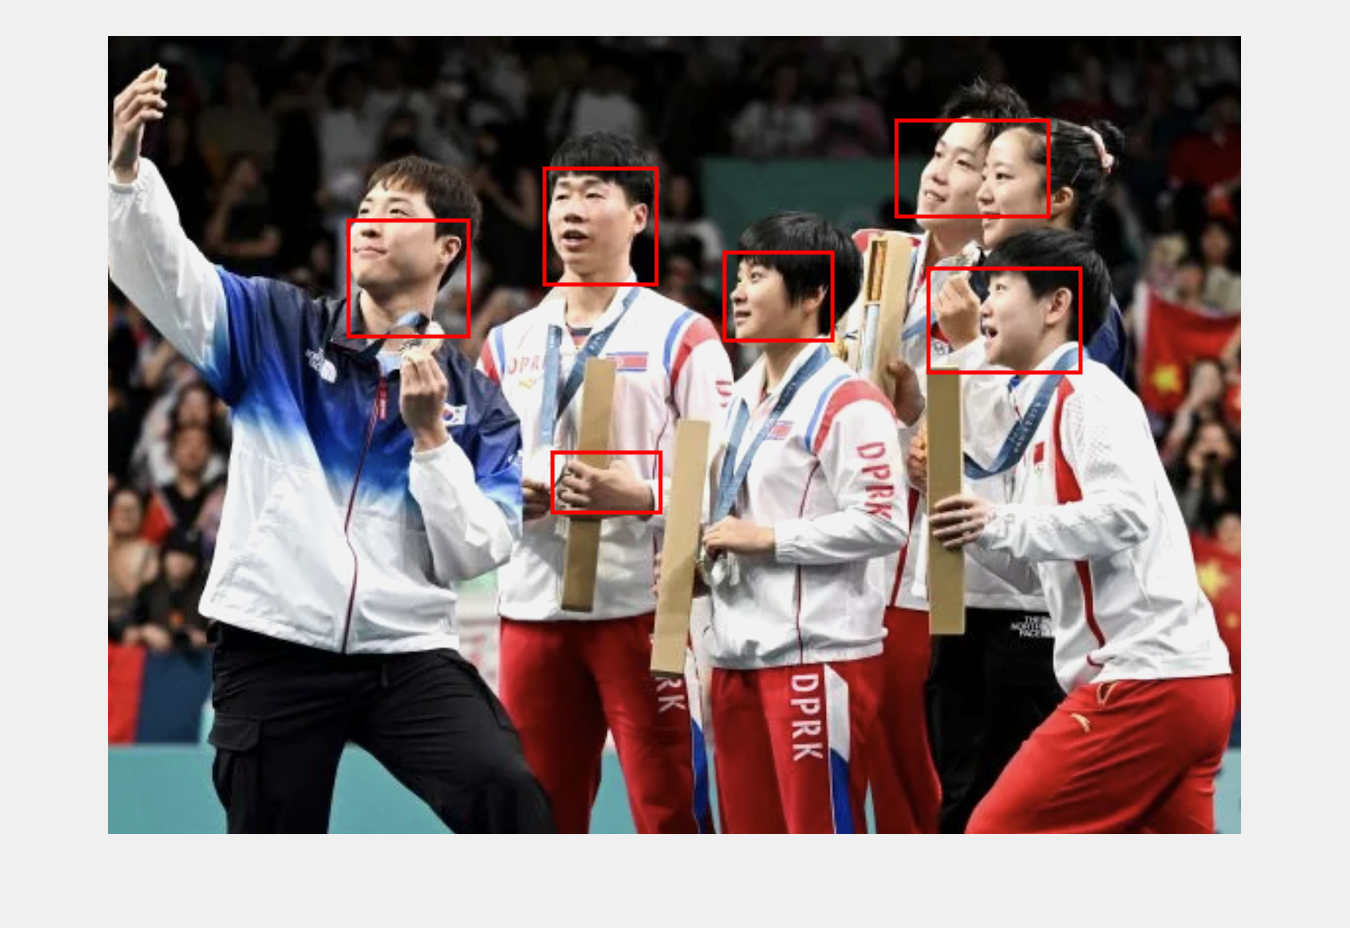
\includegraphics[width=\textwidth]{asserts/4_2_tabletennis_L3.png}
        \caption{
            L = 3, threshold = 0.475
        }\label{fig:4_2_tabletennis_L3}
    \end{subfigure}
    \vfill
    \begin{subfigure}[b]{0.6\textwidth}
        \centering
        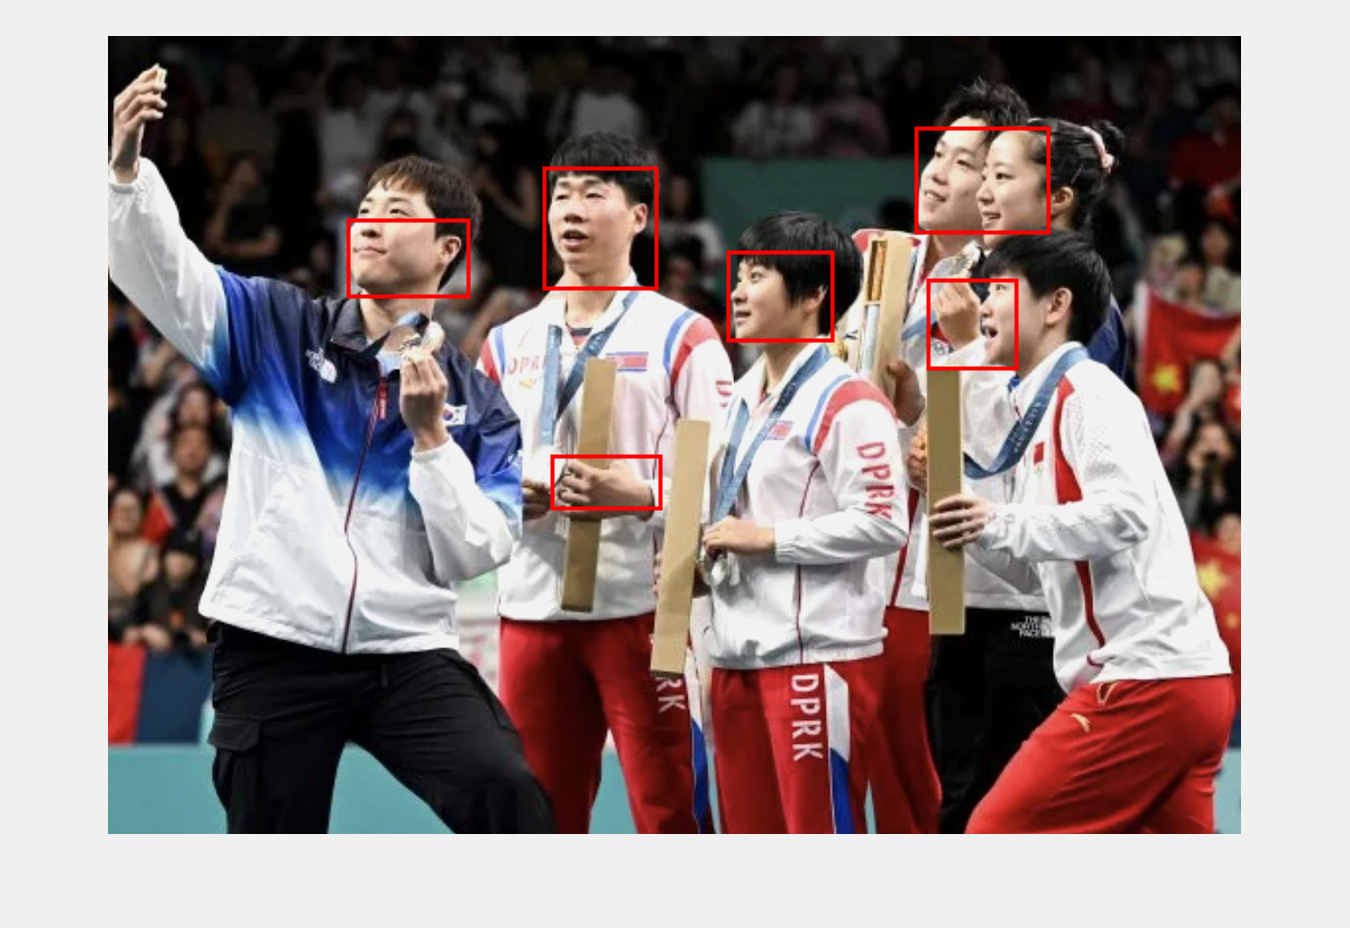
\includegraphics[width=\textwidth]{asserts/4_2_tabletennis_L4.png}
        \caption{
            L = 4, threshold = 0.625
        }\label{fig:4_2_tabletennis_L4}
    \end{subfigure}
    \vfill
    \begin{subfigure}[b]{0.6\textwidth}
        \centering
        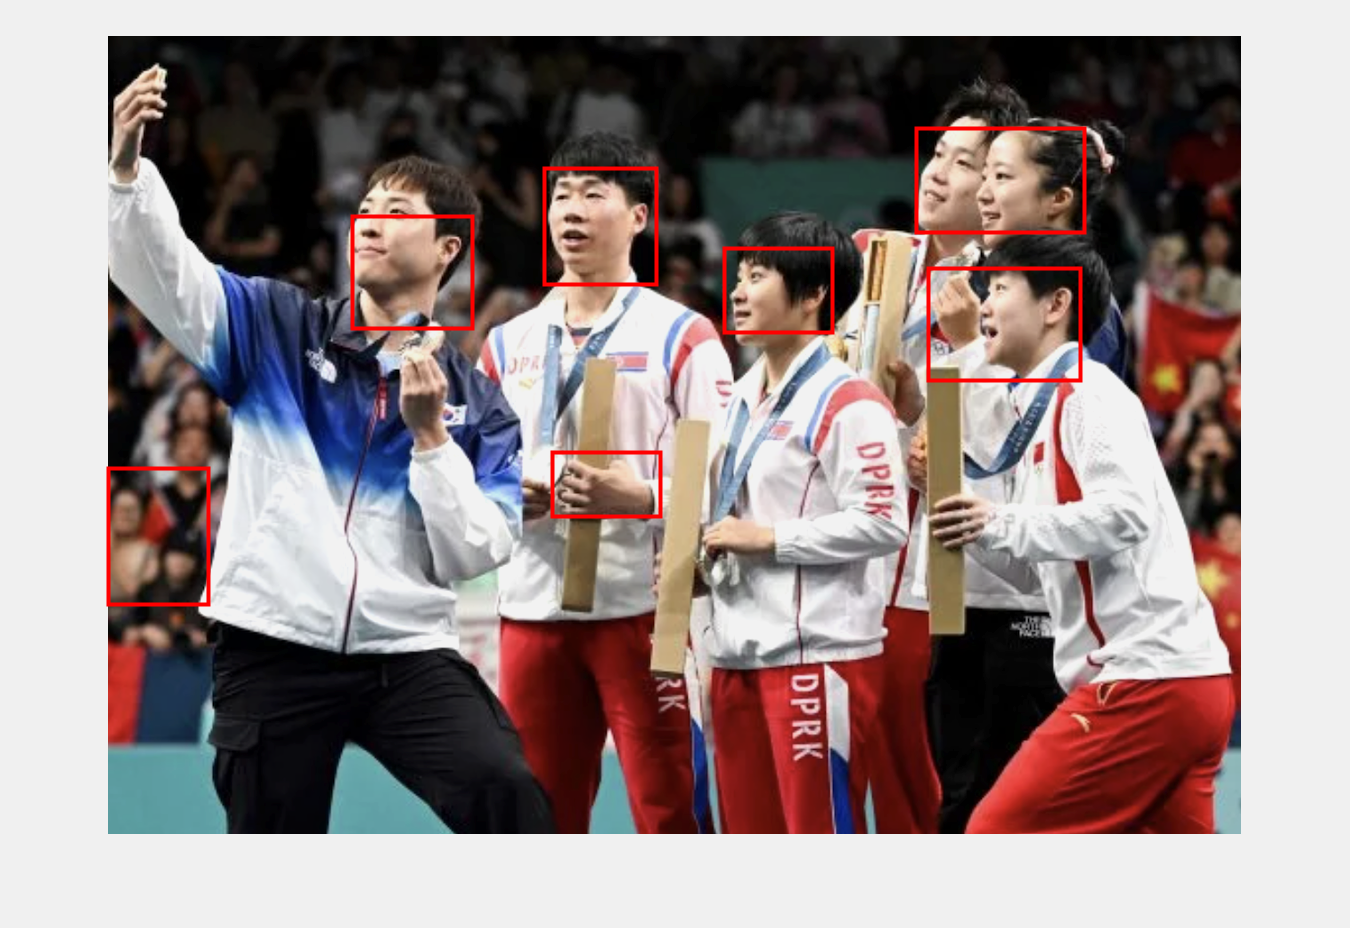
\includegraphics[width=\textwidth]{asserts/4_2_tabletennis_L5.png}
        \caption{
            L = 5, threshold = 0.795
        }\label{fig:4_2_tabletennis_L5}
    \end{subfigure}
    \caption{
        2024 巴黎奥运会朝韩乒乓球选手世纪同框自拍人脸检测结果
    }\label{fig:4_2_tabletennis}
\end{figure}

可以看到,通过调节阈值,不同的 L 均可以较好地识别出人脸。
同时,我们可以发现,这种仅依靠颜色信息的人脸检测方法无法区分贴合过近的人脸,例如图中右上角的两位选手;无法区分颜色相近、大小相近的物体,例如图中中间运动员露出的左手。

之后,我们选取 2023 年 eesast 合照作为测试图片,得到识别结果如图 \ref{fig:4_2_eesast}。

\begin{figure}[ht]
    \centering
    \begin{subfigure}[b]{1.0\textwidth}
        \centering
        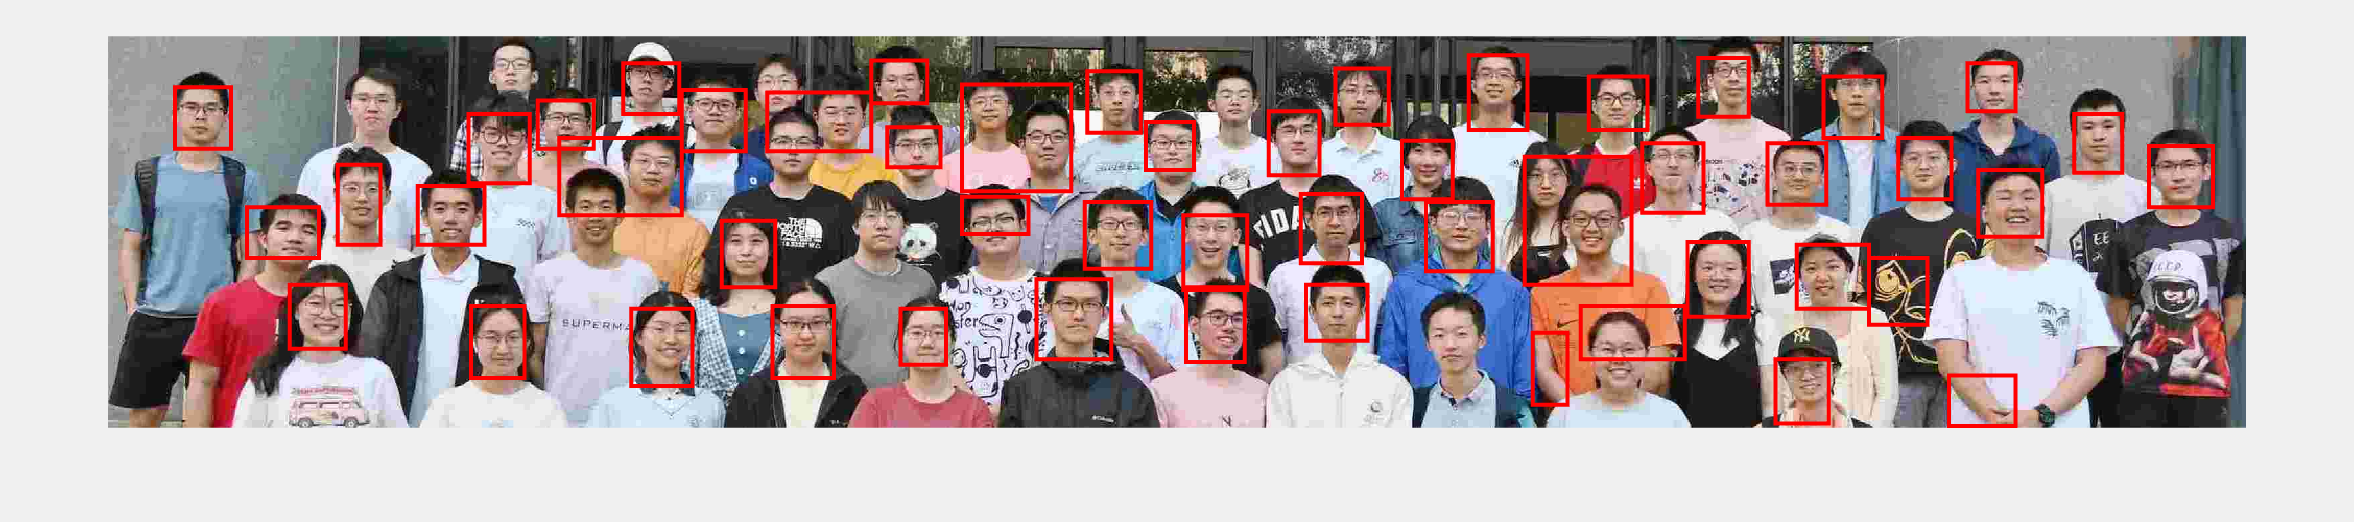
\includegraphics[width=\textwidth]{asserts/4_2_eesast_L3.png}
        \caption{
            L = 3, threshold = 0.475
        }\label{fig:4_2_eesast_L3}
    \end{subfigure}
    \vfill
    \begin{subfigure}[b]{1.0\textwidth}
        \centering
        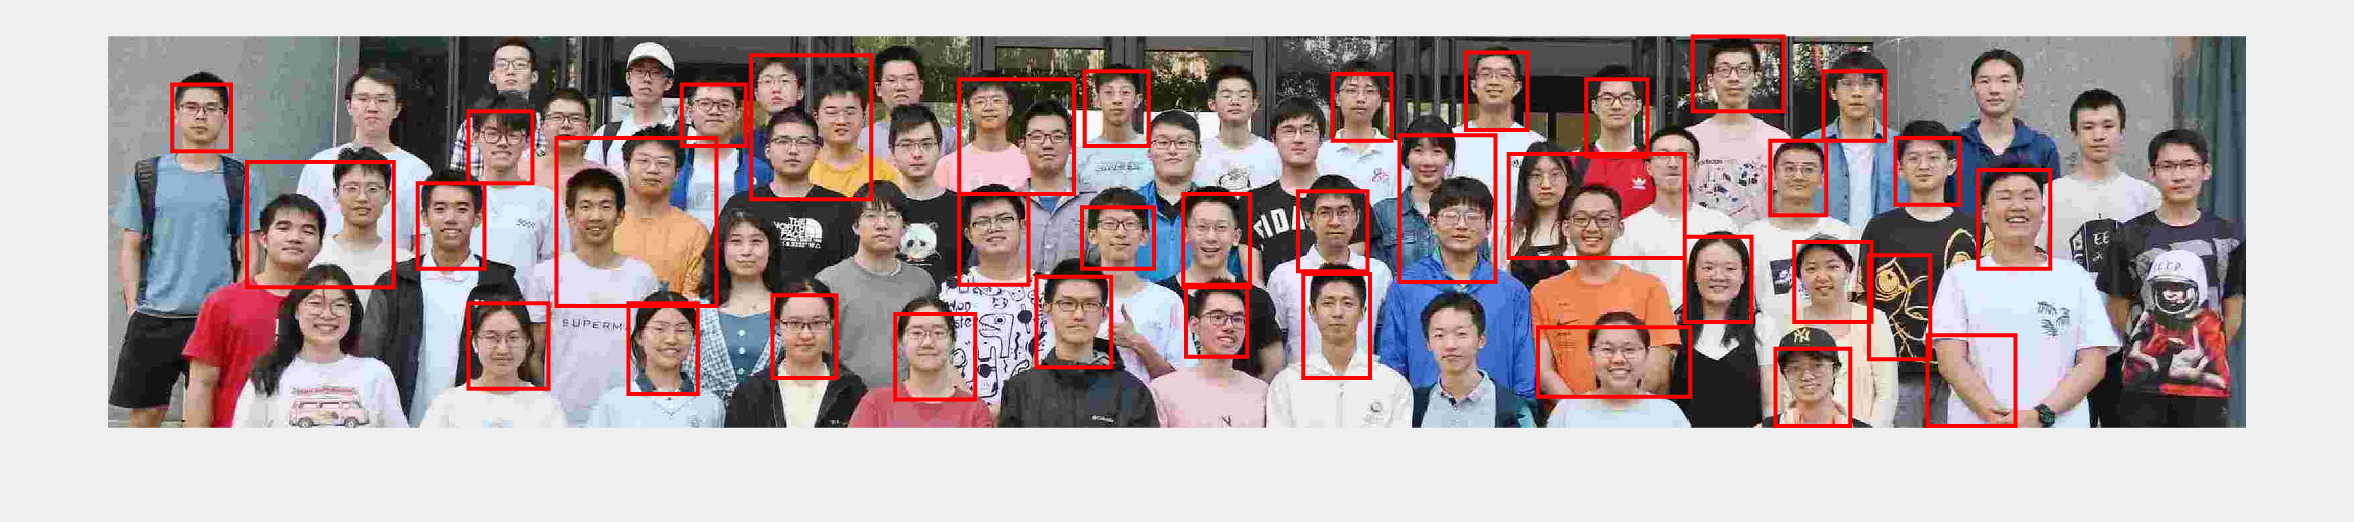
\includegraphics[width=\textwidth]{asserts/4_2_eesast_L4.png}
        \caption{
            L = 4, threshold = 0.735
        }\label{fig:4_2_eesast_L4}
    \end{subfigure}
    \vfill
    \begin{subfigure}[b]{1.0\textwidth}
        \centering
        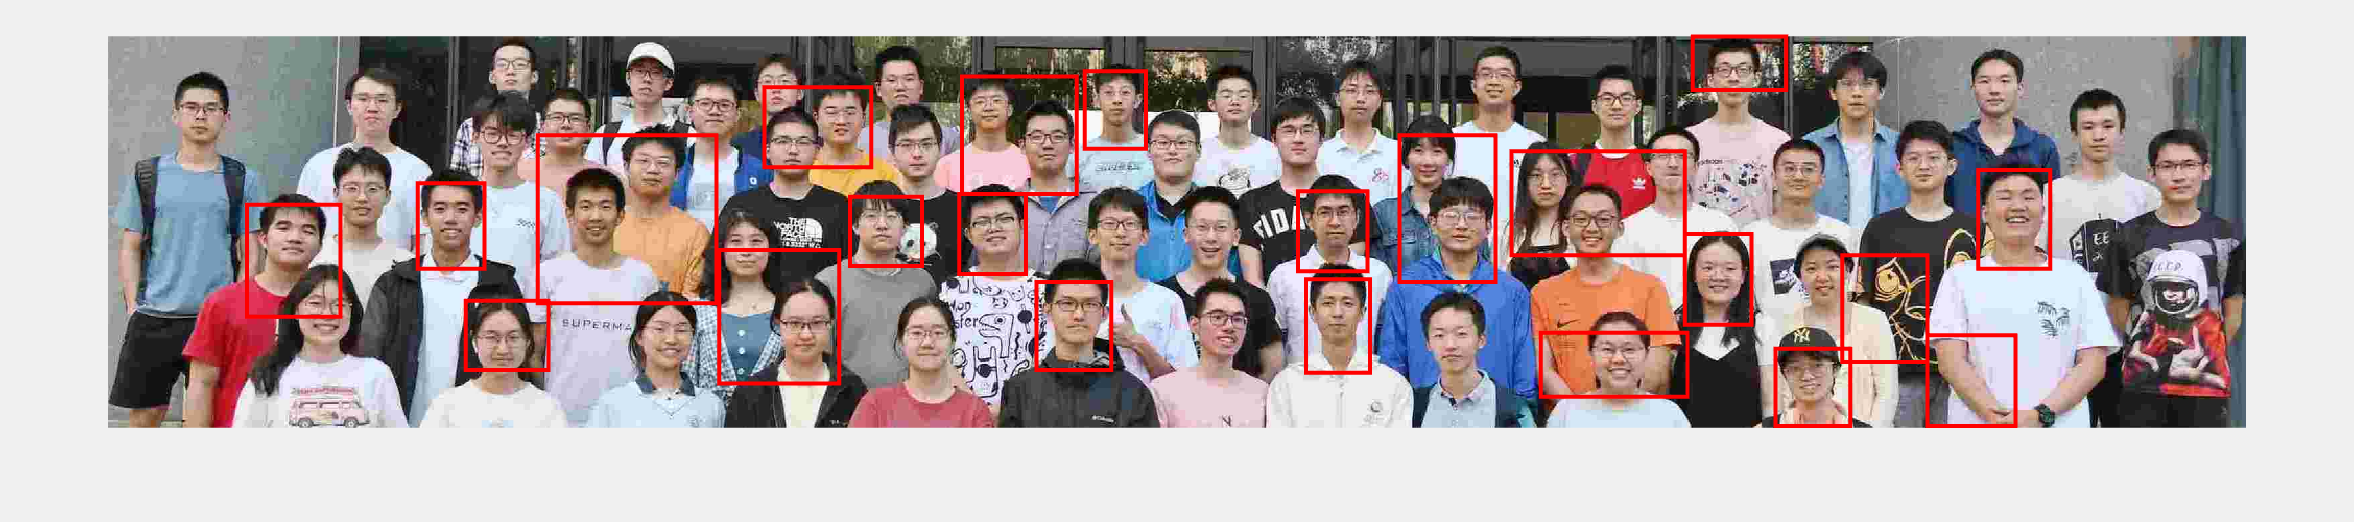
\includegraphics[width=\textwidth]{asserts/4_2_eesast_L5.png}
        \caption{
            L = 5, threshold = 0.86
        }\label{fig:4_2_eesast_L5}
    \end{subfigure}
    \caption{
        2023 年 eesast 合照人脸检测结果(未调整亮度)
    }\label{fig:4_2_eesast}
\end{figure}

当 L=3 时,采用同样的阈值可以很好地识别到大部分人脸。
但随着 L 的增大,采用相同的阈值无法很好地识别人脸。即使调整阈值,效果也不如 L=3 时好,容易出现漏检与误检的情况(如图中左边肉色衣服很容易被误检,而一些皮肤较为白皙的同学容易被漏检)。
这可能是由于测试图片的人脸颜色细节与训练图片有较大差异,例如部分肤色偏亮、不同人脸的肤色差异较大等,导致 L 较大时需要的阈值偏高;而较高的阈值容易导致背景被误检。

\subsection{图像变换后的人脸检测}

我们选取识别效果最好的 L=3 的情况,固定阈值为 0.475。

顺时针旋转 90° 后的识别结果如图 \ref{fig:4_3_eesast_2_L3}。

\begin{figure}[ht]
    \centering
    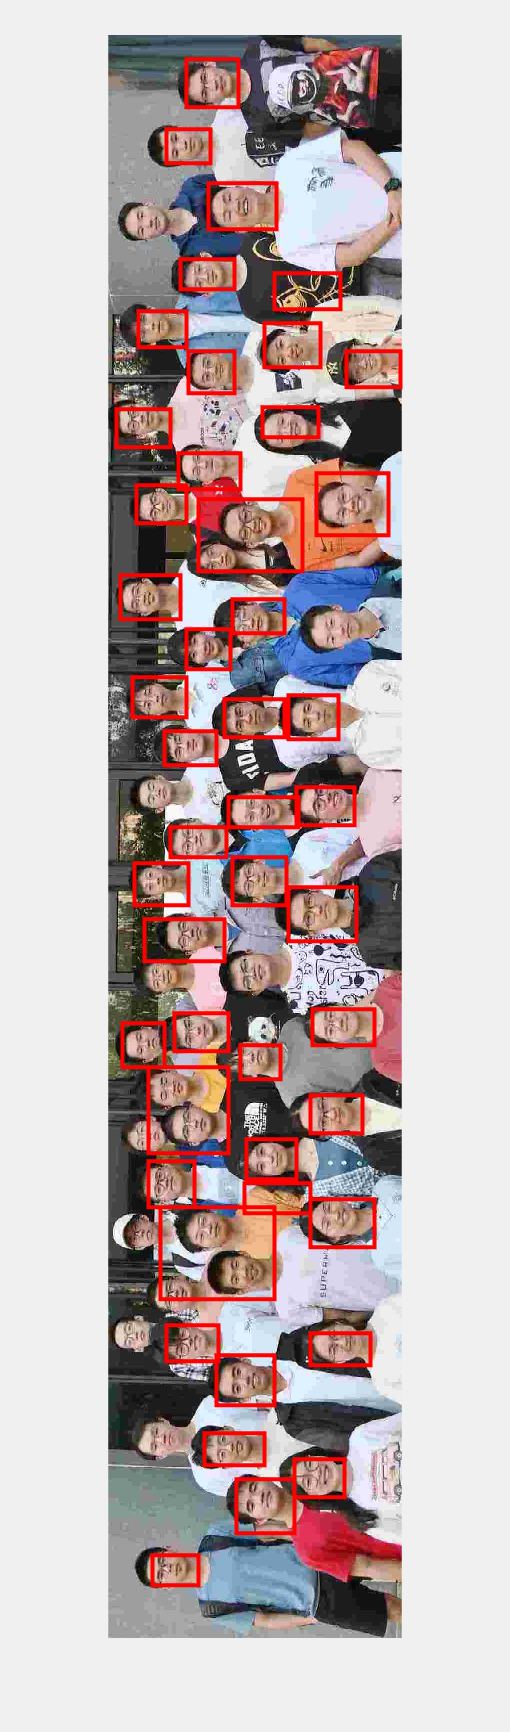
\includegraphics[width=0.3\textwidth]{asserts/4_3_eesast_2_L3.png}
    \caption{
        2023 年 eesast 合照顺时针旋转 90° 后人脸检测结果
    }\label{fig:4_3_eesast_2_L3}
\end{figure}

可见效果几乎不受影响。这可能是因为我们只关注了颜色信息,而不在意人脸的形状。

利用 \texttt{imresize} 函数将图片宽度增加一倍后的识别结果如图 \ref{fig:4_3_eesast_3_L3}。

\begin{figure}[ht]
    \centering
    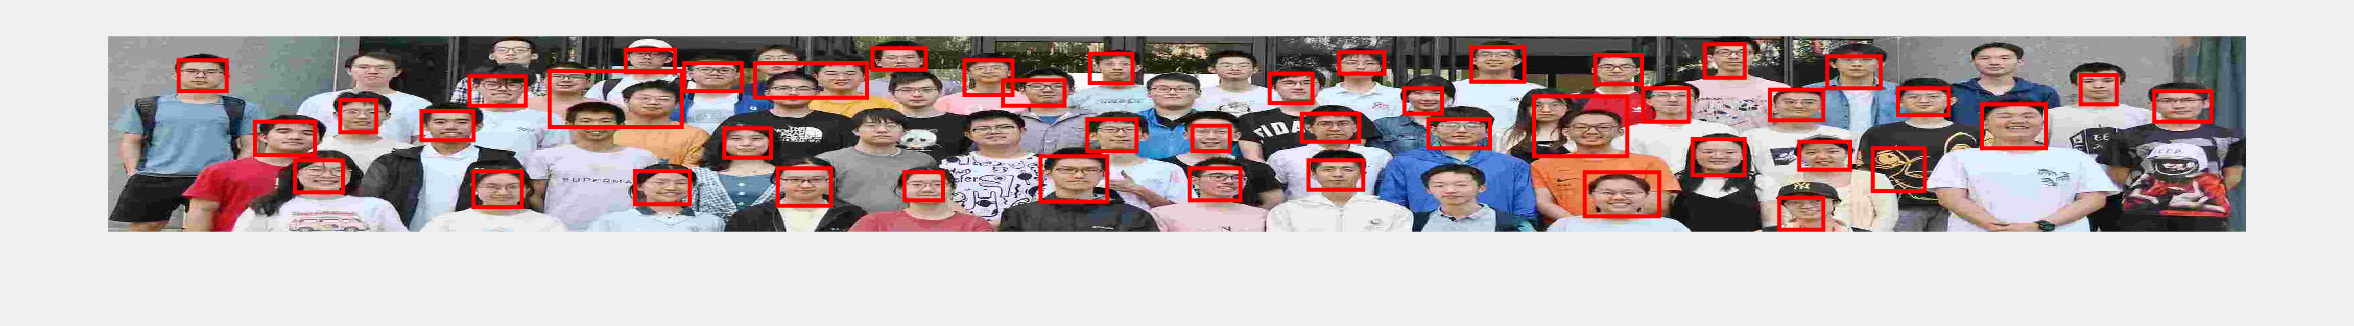
\includegraphics[width=1.0\textwidth]{asserts/4_3_eesast_3_L3.png}
    \caption{
        2023 年 eesast 合照宽度增加一倍后人脸检测结果
    }\label{fig:4_3_eesast_3_L3}
\end{figure}

可见对识别影响也不大。这说明该方法对形状变换的鲁棒性确实较好。

将图片调亮与调暗,得到识别结果如图 \ref{fig:4_3_eesast_4_L3}。

\begin{figure}[ht]
    \centering
    \begin{subfigure}[b]{1.0\textwidth}
        \centering
        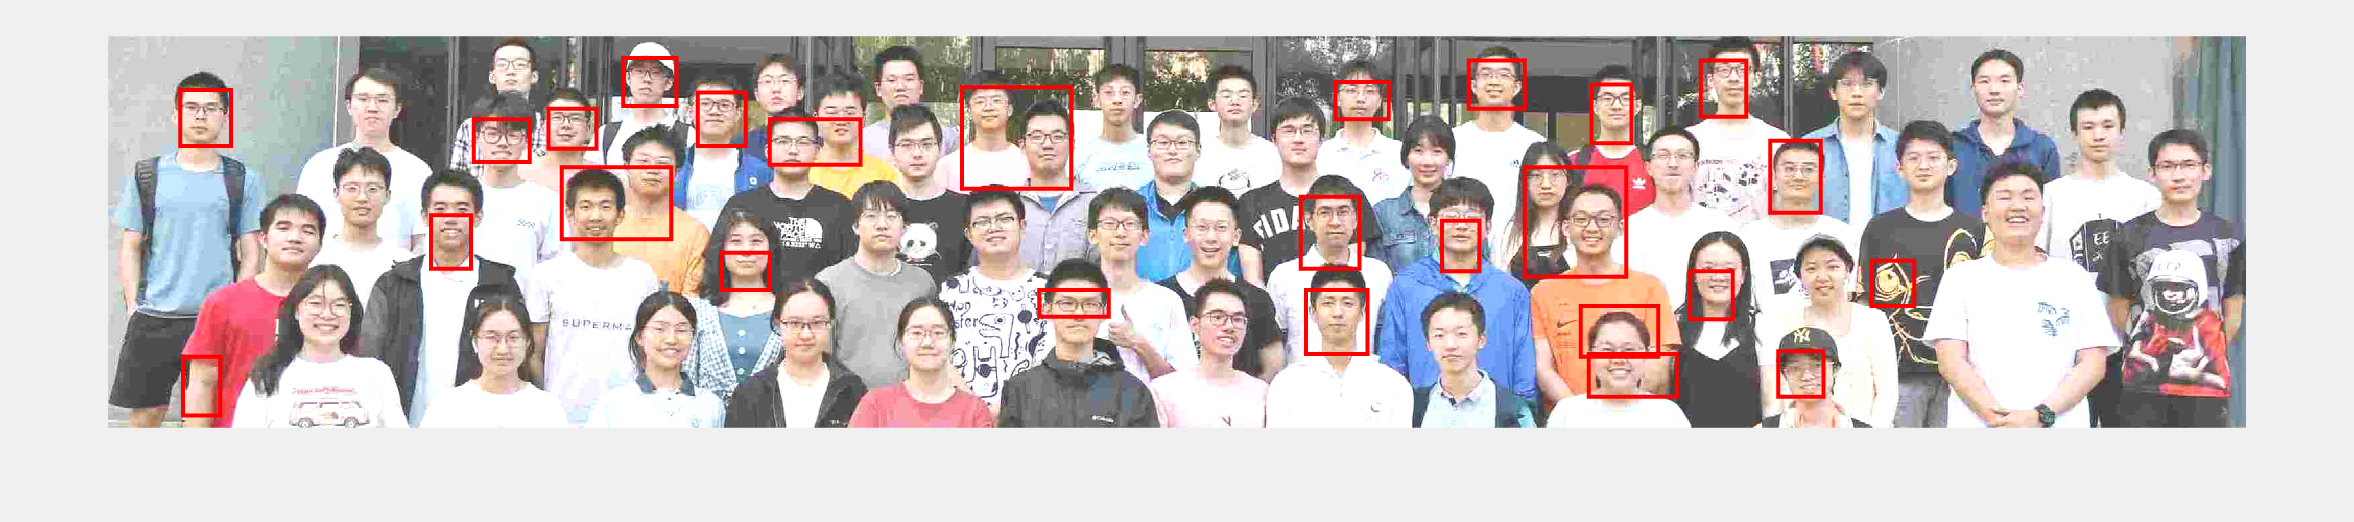
\includegraphics[width=\textwidth]{asserts/4_3_eesast_4_L3.png}
        \caption{
            2023 年 eesast 合照调亮后人脸检测结果
        }\label{fig:4_3_eesast_4_L3_1}
    \end{subfigure}
    \vfill
    \begin{subfigure}[b]{1.0\textwidth}
        \centering
        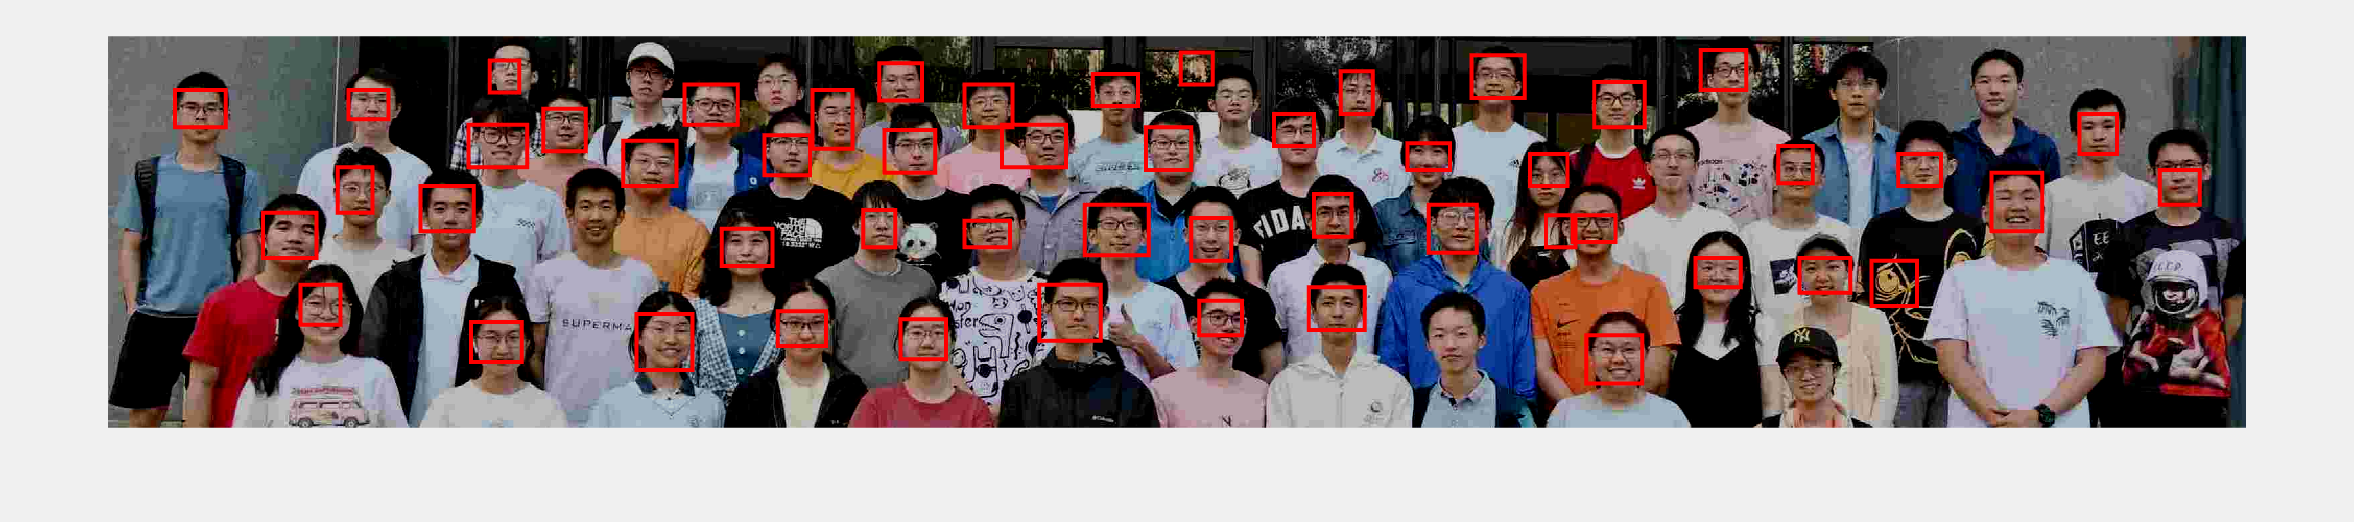
\includegraphics[width=\textwidth]{asserts/4_3_eesast_5_L3.png}
        \caption{
            2023 年 eesast 合照调暗后人脸检测结果
        }\label{fig:4_3_eesast_4_L3_2}
    \end{subfigure}
    \caption{
        2023 年 eesast 合照调亮与调暗后人脸检测结果
    }\label{fig:4_3_eesast_4_L3}
\end{figure}

可见调亮后识别效果较差,而调暗后识别效果很好。
这印证了之前的猜想:该测试图片相较于训练图片,亮度更低,识别难度更大。

首次启发,我用降低了亮度的图片再次进行了实验,得到识别结果如图 \ref{fig:4_4_eesast}。

\begin{figure}[ht]
    \centering
    \begin{subfigure}[b]{1.0\textwidth}
        \centering
        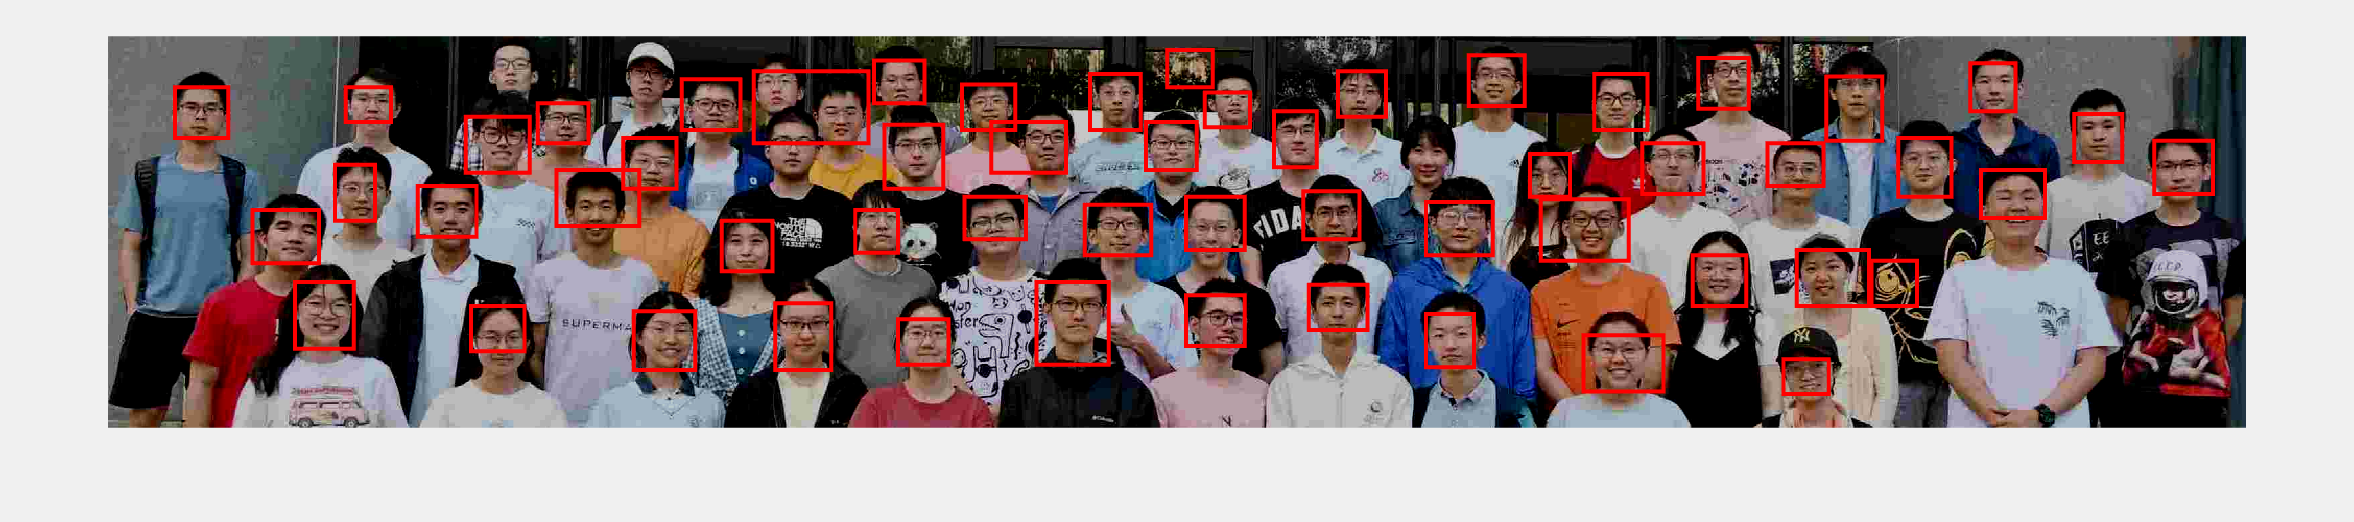
\includegraphics[width=\textwidth]{asserts/4_4_eesast_L3.png}
        \caption{
            L = 3, threshold = 0.525
        }\label{fig:4_4_eesast_L3}
    \end{subfigure}
    \vfill
    \begin{subfigure}[b]{1.0\textwidth}
        \centering
        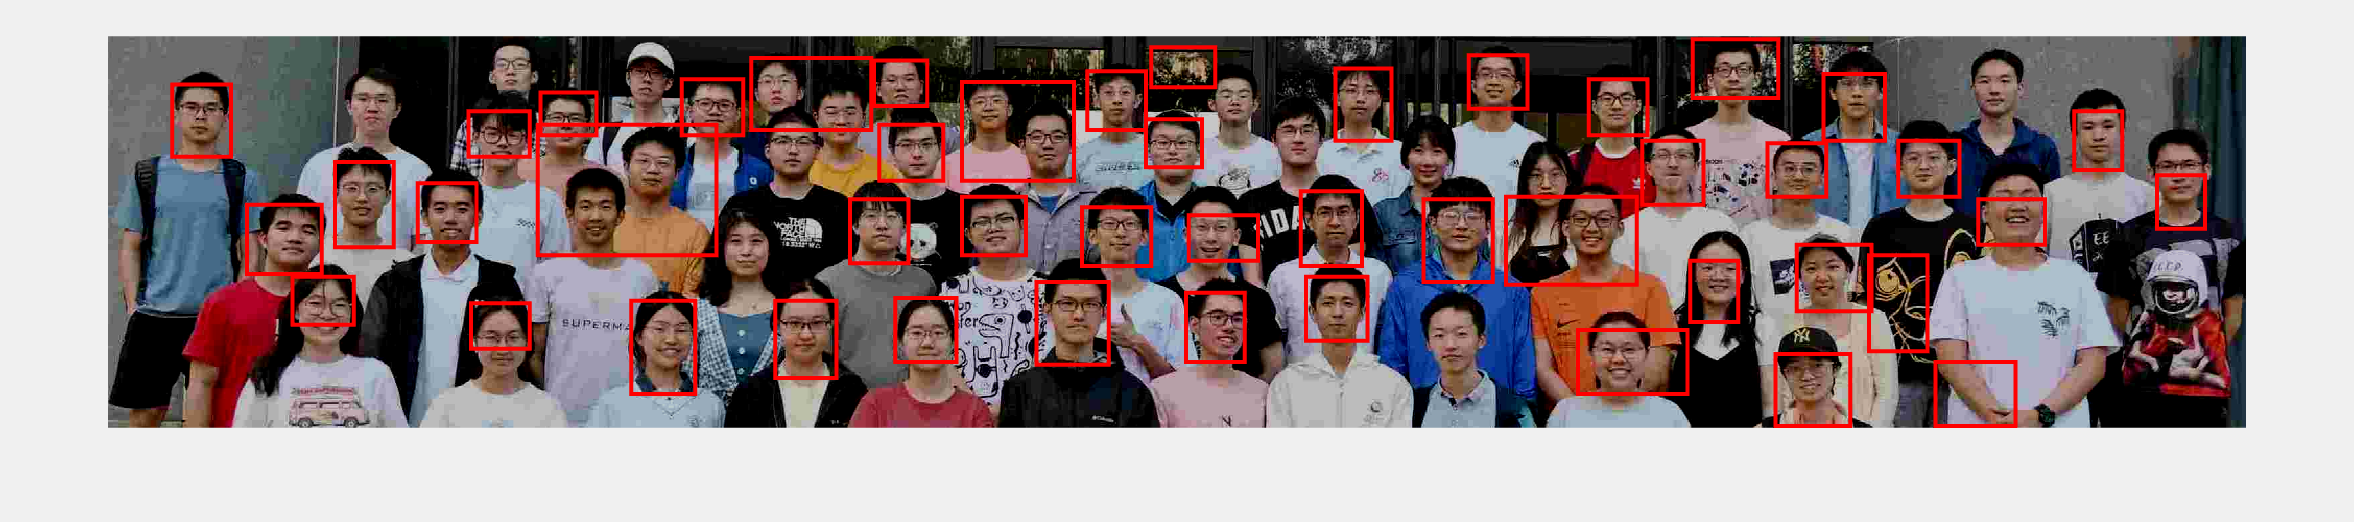
\includegraphics[width=\textwidth]{asserts/4_4_eesast_L4.png}
        \caption{
            L = 4, threshold = 0.735
        }\label{fig:4_4_eesast_L4}
    \end{subfigure}
    \vfill
    \begin{subfigure}[b]{1.0\textwidth}
        \centering
        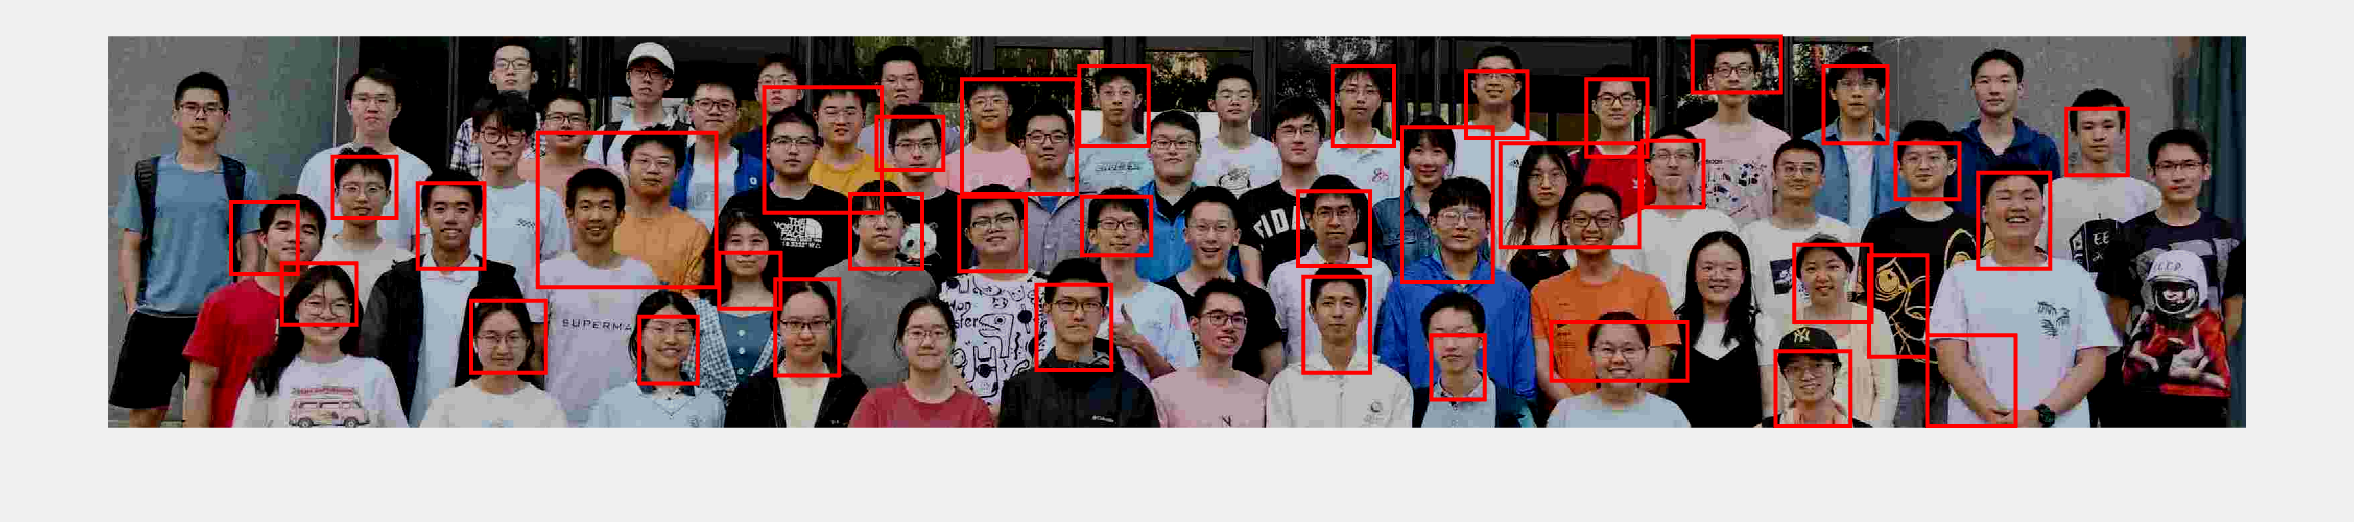
\includegraphics[width=\textwidth]{asserts/4_4_eesast_L5.png}
        \caption{
            L = 5, threshold = 0.87
        }\label{fig:4_4_eesast_L5}
    \end{subfigure}
    \caption{
        2023 年 eesast 合照人脸检测结果(亮度调整)
    }\label{fig:4_4_eesast}
\end{figure}

可以看到,降低亮度后,不同的 L 值识别效果均明显得到提升,其中 L=3 时达到了相当高的准确率。
这说明基于颜色信息的人脸检测确实严重依赖于亮度信息,提示我们实际应用时需要配合其它特征。

\subsection{重新选择人脸样本训练标准}

从实验中我们可以发现,根据颜色信息的人脸识别对人脸形状鲁棒,但对肤色亮度敏感,且容易受相近颜色背景干扰,例如人的手部或肉色衣物。

因此,我认为除了颜色,还需综合考虑其它特征,例如形状、纹理等。
可能的方法是对颜色求梯度,提取梯度特征,即轮廓特征;或者对颜色进行聚类,提取聚类特征。
综合多种特征,预期可以提高人脸识别的准确性,降低误检率。

\section{实验总结}

本次实验主要研究了图像处理的基本原理和方法,实现了 JPEG 编码解码、基于颜色信息的人脸检测等实验。

除此以外,实验中多次尝试提高代码的效率,通过实验掌握了一些小技巧,例如避免重复分配内存、避免循环中的重复计算等,积累了一些经验。

所有代码均位于 \texttt{src} 目录下,可供查阅。

\end{document}